\documentclass[9pt]{beamer}

%!TEX root = ../notas_de_clase.tex

%preamble

%language
\usepackage[spanish,es-nodecimaldot]{babel}
\usepackage[utf8]{inputenc}
\usepackage{apacite}
\usepackage[absolute,overlay]{textpos}

%packages
\usepackage[Algoritmo]{algorithm}
\usepackage{algorithmicx}
\usepackage[noend]{algpseudocode}
\usepackage{mathtools}
\setlength {\marginparwidth}{2cm}
\usepackage{todonotes}
\usepackage{amsbsy}
\usepackage{amssymb}
\usepackage{amsmath,bm}
\usepackage{dsfont}

\usepackage{comment}

\usepackage{xcolor}
\providecommand{\sred}[1]{\textcolor{red}{#1}}
\providecommand{\sblue}[1]{\textcolor{blue}{#1}}
\providecommand{\red}[1]{\textcolor{red}{\text{#1}}}
\providecommand{\blue}[1]{\textcolor{blue}{\text{#1}}}
\providecommand{\redb}[1]{\textcolor{red}{\textbf{#1}}}
\providecommand{\blueb}[1]{\textcolor{blue}{\textbf{#1}}}
\usepackage{graphicx}
\usepackage{fancybox}
\usepackage{booktabs}
\usepackage{caption}
\usepackage{float}
%\usepackage[longend,ruled,algochapter,linesnumbered,lined,boxed,commentsnumbered,spanish]{algorithm2e}
%\usepackage[algo2e]{algorithm2e}
\usepackage{amssymb}
\usepackage{amstext}
\usepackage{bm}
\usepackage{wrapfig}
\usepackage{subcaption} % para_unsupervised_chapter

%formatting

\usepackage[export]{adjustbox}

%caption para figuras
\captionsetup[figure]{width=.8\linewidth, font=small,labelfont={bf},name={Fig.},labelsep=period}
\captionsetup[table]{width=.8\linewidth,font=small,labelfont={bf},name={Tabla},labelsep=period}



\ifx\byn\undefined
    \definecolor{my_blue}{HTML}{C2D5FF}
    \definecolor{my_red}{HTML}{FFC2C2}
    \definecolor{my_yellow}{HTML}{FFFFE0}
\else
    \definecolor{my_blue}{HTML}{FFFFFF}
    \definecolor{my_red}{HTML}{FFFFFF}
    \definecolor{my_yellow}{HTML}{FFFFFF}
\fi


\usepackage[framemethod=TikZ]{mdframed}
\mdfdefinestyle{discusion}{%
    %linecolor=black,
    %outerlinewidth=0pt,
    roundcorner=0pt,
    innertopmargin=5pt,
    innerbottommargin=5pt,
    innerrightmargin=20pt,
    innerleftmargin=20pt,
    backgroundcolor=my_blue}

\colorlet{Green}{green!90}


\mdfdefinestyle{ejemplo}{%
    %linecolor=black,
    %outerlinewidth=0pt,
    roundcorner=0pt,
    innertopmargin=5pt,
    innerbottommargin=5pt,
    innerrightmargin=20pt,
    innerleftmargin=20pt,
    backgroundcolor=my_yellow}


\mdfdefinestyle{pendiente}{%
    style = discusion, 
    backgroundcolor=my_red}


\RequirePackage{url}



%definitions
\def\td{{\text d}}
\def\cN{{\mathcal N}}
\def\cX{{\mathcal X}} 
\def\cC{{\mathcal C}} 
\def\N{{\mathbb N}}
\def\d{{\text d}}
\def\datos{{\mathcal D}}
\def\eye{{\mathbb I}}
\def\ssum{{\scriptstyle\sum}}
\def\bepsilon{{\bm \epsilon}}
\def\tx{\tilde{x}}
\def\tX{\tilde{X}}
\def\thetaMAP{\theta_\text{MAP}}
\newcommand{\gp}{\ensuremath{\mathcal{GP}}}
\newcommand{\pr}{\ensuremath{\mathbb{P}}}
\newcommand{\x}{\ensuremath{\mathbf{x}}}
\newcommand{\z}{\ensuremath{\mathbf{z}}}
\newcommand{\cvector}{\ensuremath{\mathbf{c}}}
\newcommand{\e}{\ensuremath{\mathbf{e}}}
\newcommand{\y}{\ensuremath{\mathbf{y}}}
\newcommand{\bx}{\ensuremath{\textcolor{blue}{X}}}
\newcommand{\by}{\ensuremath{\textcolor{blue}{Y}}}
\newcommand{\rx}{\ensuremath{\textcolor{red}{X_*}}}

\newcommand{\R}{\mathbb{R}}
\newcommand{\norm}[1]{\left\lVert#1\right\rVert}




\DeclareMathOperator*{\argmax}{arg\,max}
\DeclareMathOperator*{\argmin}{arg\,min}
\DeclareMathOperator{\E}{\mathbb{E}}
\DeclareMathOperator{\V}{\mathbb{V}}
\DeclareMathOperator{\KL}{\text{KL}}
\DeclareMathOperator{\MVN}{\text{MVN}}
\newcommand\deq{\stackrel{\mathclap{\normalfont\mbox{\tiny def}}}{=}}
%\newcommand{\E}[1]{\mathbb E \left[#1\right]}
\newcommand{\trace}[1]{\text{Tr} \left[#1\right]}


\usepackage{amsthm}

%-------------------------------------------
% Newtheorem
%-------------------------------------------
\newtheorem{axioma}{\textcolor{red}{Axioma}}
\newtheorem{definicion}{Definición}
\newtheorem*{notacion}{Notación}
\newtheorem{teorema}{Teorema}
\newtheorem{corolario}{Corolario}
\newtheorem{lema}{Lema}
\newtheorem{lemaZ}{\textcolor{red}{Lema}}
\newtheorem{propiedad}{Propiedad:}
\newtheorem{proposicion}{Proposición:}
\newtheorem*{observacion}{Observación}
\newtheorem*{comentario}{Comentario}
\newtheorem*{ejemplo}{Ejemplo}
\newtheorem*{resultado}{Resultado}
\newtheorem*{propuesto}{Ejercicio propuesto}
\newtheorem*{demostracion}{Demostración} % No se usa, usar \begin{proof}\end{proof} que son por default.

%listing paackage para código
\usepackage{listings}
\usepackage{xcolor}
 
\definecolor{codegreen}{rgb}{0,0.6,0}
\definecolor{codegray}{rgb}{0.5,0.5,0.5}
\definecolor{codepurple}{rgb}{0.58,0,0.82}
\definecolor{backcolour}{rgb}{0.95,0.95,0.92}
 
\lstdefinestyle{mystyle}{
    xleftmargin=0.15\textwidth,
    linewidth=0.8\textwidth,
    backgroundcolor=\color{backcolour},   
    commentstyle=\color{codegreen},
    keywordstyle=\color{magenta},
    numberstyle=\tiny\color{codegray},
    stringstyle=\color{codepurple},
    basicstyle=\ttfamily\footnotesize,
    breakatwhitespace=true,         
    breaklines=true,                 
    captionpos=b,                    
    keepspaces=true,                 
    numbers=left,                    
    numbersep=5pt,                  
    showspaces=false,                
    showstringspaces=false,
    showtabs=false,                  
    tabsize=2
}
 
\lstset{style=mystyle}

\numberwithin{equation}{section}

\usetheme{simple}
\usepackage{tikz}

\title{Clase 7: Modelos Auto-regresivos}
\subtitle{MDS7203 Modelos Generativos Profundos}
\date{22 de septiembre 2023}
\author{Felipe Tobar \\ Cristóbal Alcázar - Camilo Carvajal Reyes}  
\titlegraphic{
\begin{tikzpicture}[remember picture, overlay]
    \node[opacity=1.0, at=(current page.center)] {
\includegraphics[width=\paperwidth,height=\paperheight]{diapositivas/img/presentacion_plantilla_4_fondo_blanco-celeste.png}};
\end{tikzpicture}
\begin{figure}[htp] 
    \centering
        
\includegraphics[width=0.15\textwidth]{img/Uchile.pdf}%
        \hspace{1cm}
        \includegraphics[width=0.15\textwidth]{diapositivas/img/IDIA.png}
\end{figure}
}
\institute{Iniciativa de Datos e Inteligencia Artificial\\Universidad de Chile}

\begin{document}
\begin{frame}
  \titlepage
\end{frame}

\begin{frame}
    \frametitle{Tabla de contenidos}
    \tableofcontents
\end{frame}


\section{NLP and language models}
\begin{frame}
    \frametitle{Table of contents}
    \tableofcontents[currentsection]
\end{frame}

%\subsection{NLP and its applications}
\subsection{NLP, applications and challenges}
\begin{frame}{What is NLP?}
\vspace{0.3cm}\\
\begin{columns}[onlytextwidth]
    \begin{column}{0.40\textwidth}
        \textbf{Natural Language Processing} is a sub-field of linguistics, computer science and artificial intelligence, that connects computers and human language. %Sometimes it is also called \textbf{Computational Linguistics}, although
        \vspace{0.3cm} \\The field has experienced major changes since recent growth of \textbf{Deep Learning}.
    \end{column}
    \begin{column}{0.60\textwidth}
        \begin{figure}
            \centering
            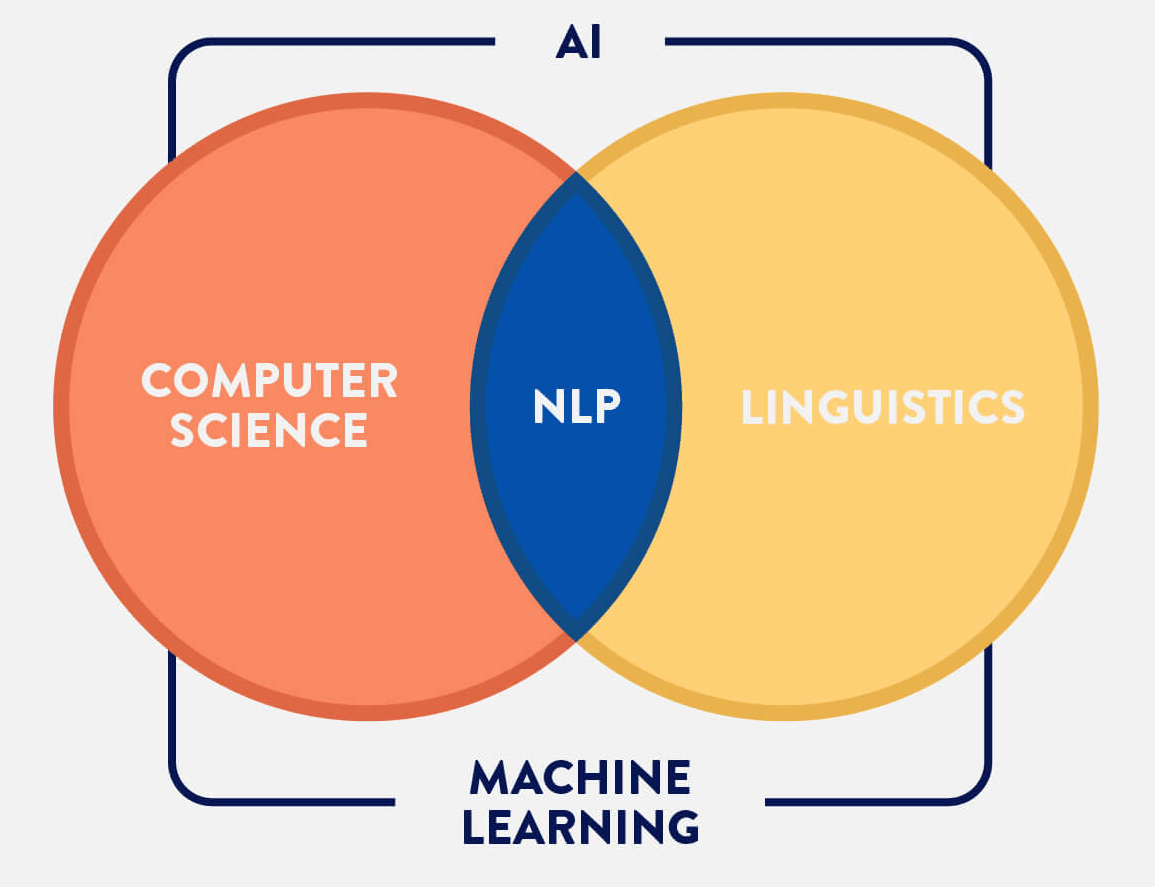
\includegraphics[width = 6.5cm]{img/natural-language-processing.png}
            \label{fig:enter-label}
        \end{figure}
         %\begin{textblock}{0.6}(0.45, 0.25)
        %     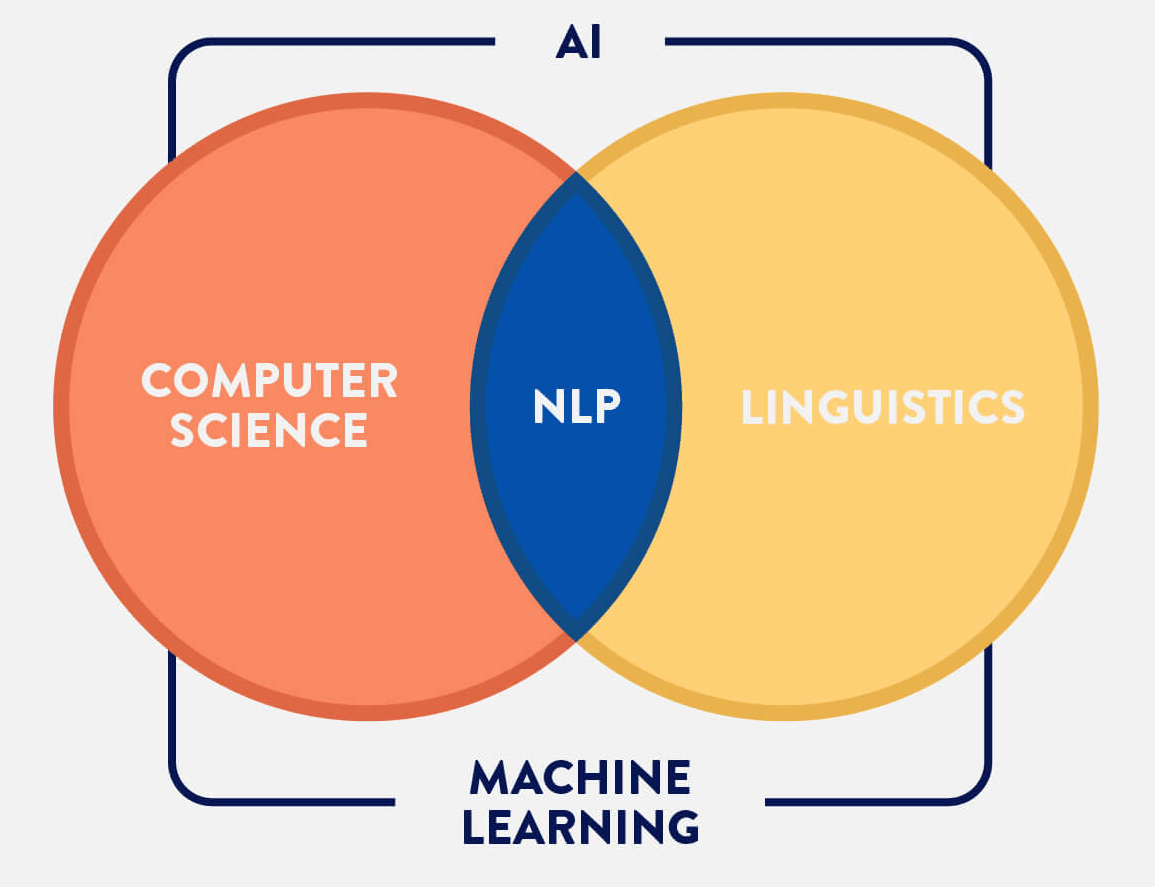
\includegraphics[width = 6.5cm]{img/natural-language-processing.png}
        % \end{textblock}
    \end{column}
\end{columns}
\end{frame}


\iffalse
\begin{frame}{Why bothering at all with NLP?}
\begin{columns}[onlytextwidth]
    \begin{column}{0.50\textwidth}
    Computational encoding of text opens the gate for:
    \begin{itemize}
        \item Machine Translation
        \only <2,3,4,5>{
        \item Natural Language Understanding
        \item Automatic Text Summarisation}
        \only <3,4,5>{
        \item Computational Linguistics}
        \only <4,5>{
        \item Natural Language Generation
        \item Question-Answering}
        \only <5>{
        \item Sentiment Analysis}
    \end{itemize}
    \end{column}
\end{columns}
\only <1> {
\begin{textblock}{0.5}(0.55, 0.25)
        \includegraphics[width = 5cm]{img/machine_translation.png}
\end{textblock}}
\only <2> {
\begin{textblock}{0.5}(0.55, 0.35)
        \includegraphics[width = 5cm]{img/text_summarisation.png}
\end{textblock}}
\only <3> {
\begin{textblock}{0.5}(0.55, 0.25)
        \includegraphics[width = 5cm]{img/parse_tree.png}
\end{textblock}}
\only <4> {
\begin{textblock}{0.5}(0.55, 0.25)
        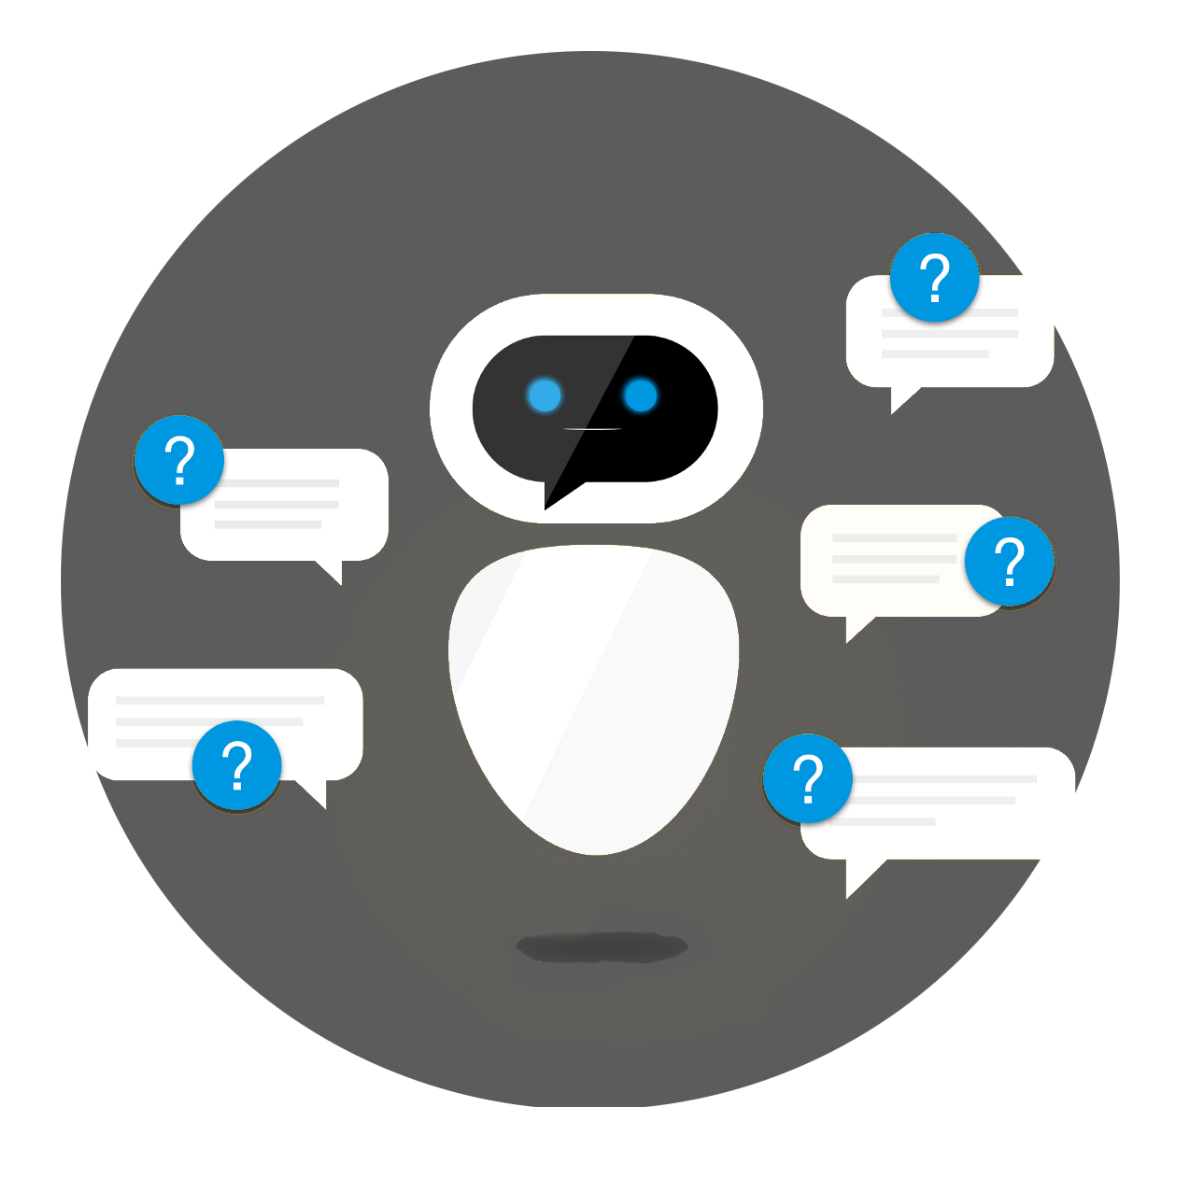
\includegraphics[width = 5cm]{img/question_answering.png}
\end{textblock}
}
\only <5> {
\begin{textblock}{0.5}(0.55, 0.25)
        \includegraphics[width = 5cm]{img/sentiment_anlysis.png}
\end{textblock}}
\end{frame}
\fi

\begin{frame}{Why bothering at all with NLP?}
\begin{columns}[onlytextwidth]
    \begin{column}{0.50\textwidth}
    Computational encoding of text opens the gate for:
    \begin{itemize}
        \item Machine Translation
        \item Natural Language Understanding
        \item Automatic Text Summarisation
        \item Computational Linguistics
        \item Natural Language Generation
        \item Question-Answering
        \item Sentiment Analysis
    \end{itemize}
    \end{column}
    \begin{column}{0.50\textwidth}
        \begin{figure}
            \centering
            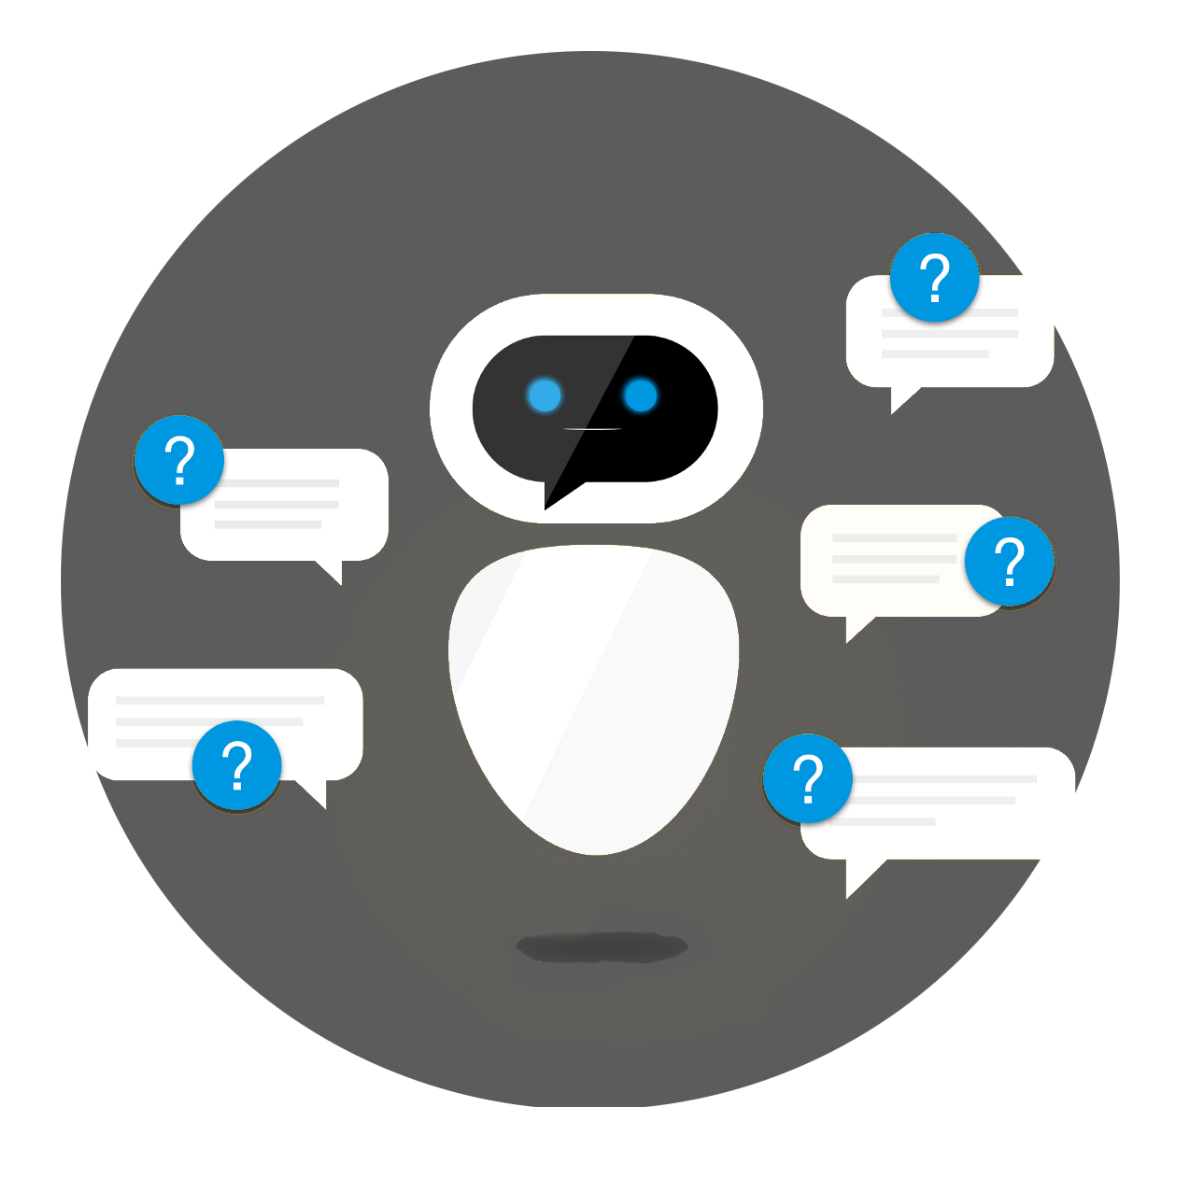
\includegraphics[width = 5cm]{img/question_answering.png}
            % \caption{Caption}
            % \label{fig:enter-label}
        \end{figure}
    \end{column}
\end{columns}
\end{frame}

%\subsection{Challenges of NLP}
\iffalse
\begin{frame}{Representation of text}
\textbf{Differences with Image and Audio processing}
\begin{columns}[onlytextwidth]
    \begin{column}{0.50\textwidth}
    With both images and audio, we start from a \textbf{signal}.\\
    That signal is often of little use without some appropriate pre-processing.
    \vspace{0.5cm}\\
    \only <2> {However, this isn't the case for text.
    \vspace{0.5cm}\\ Hence, the \textbf{representation learning} process happens from scratch}
    \end{column}
\end{columns}
\only <1> {
\begin{textblock}{0.5}(0.55, 0.25)
        \includegraphics[width = 5.2cm]{img/image_processing.png}
\end{textblock}
\begin{textblock}{0.5}(0.55, 0.55)
        \includegraphics[width = 5cm]{img/audio_processing.png}
\end{textblock}}
\only <2> {
\begin{textblock}{0.5}(0.55, 0.25)
    \includegraphics[width = 5.2cm]{img/NLP_figure1.png}
\end{textblock}}
\end{frame}
\fi


\begin{frame}{Representation of text}
\begin{columns}[onlytextwidth]
    \begin{column}{0.50\textwidth}
    \vspace{0.3cm}\\
    \only <1> {\textbf{One hot-encoding} \\ It is one possible approach for giving a vector to a word. Let's consider a vocabulary of possible words $V$ with $n$ terms. A one-hot representation for the word $w$, indexed by $i$ in the vocabulary will correspond to the vector that has only zeros, except for the position $i$. That way, we can distinguish two different words.}
    \only <2> {\textbf{Bag-of-words} \\ Corresponds to a document representation in which we add up the corresponding one hot-encoding vectors. The result is an $n$-dimensional vector with the frequency of each word.
    
    We may also consider a \textbf{vector of occurrence}, in which the $i$-th position has $1$ if the word is in the document, regardless of the repetitions}
    \end{column}
    \begin{column}{0.50\textwidth}
        \centering
        \only <1> {
            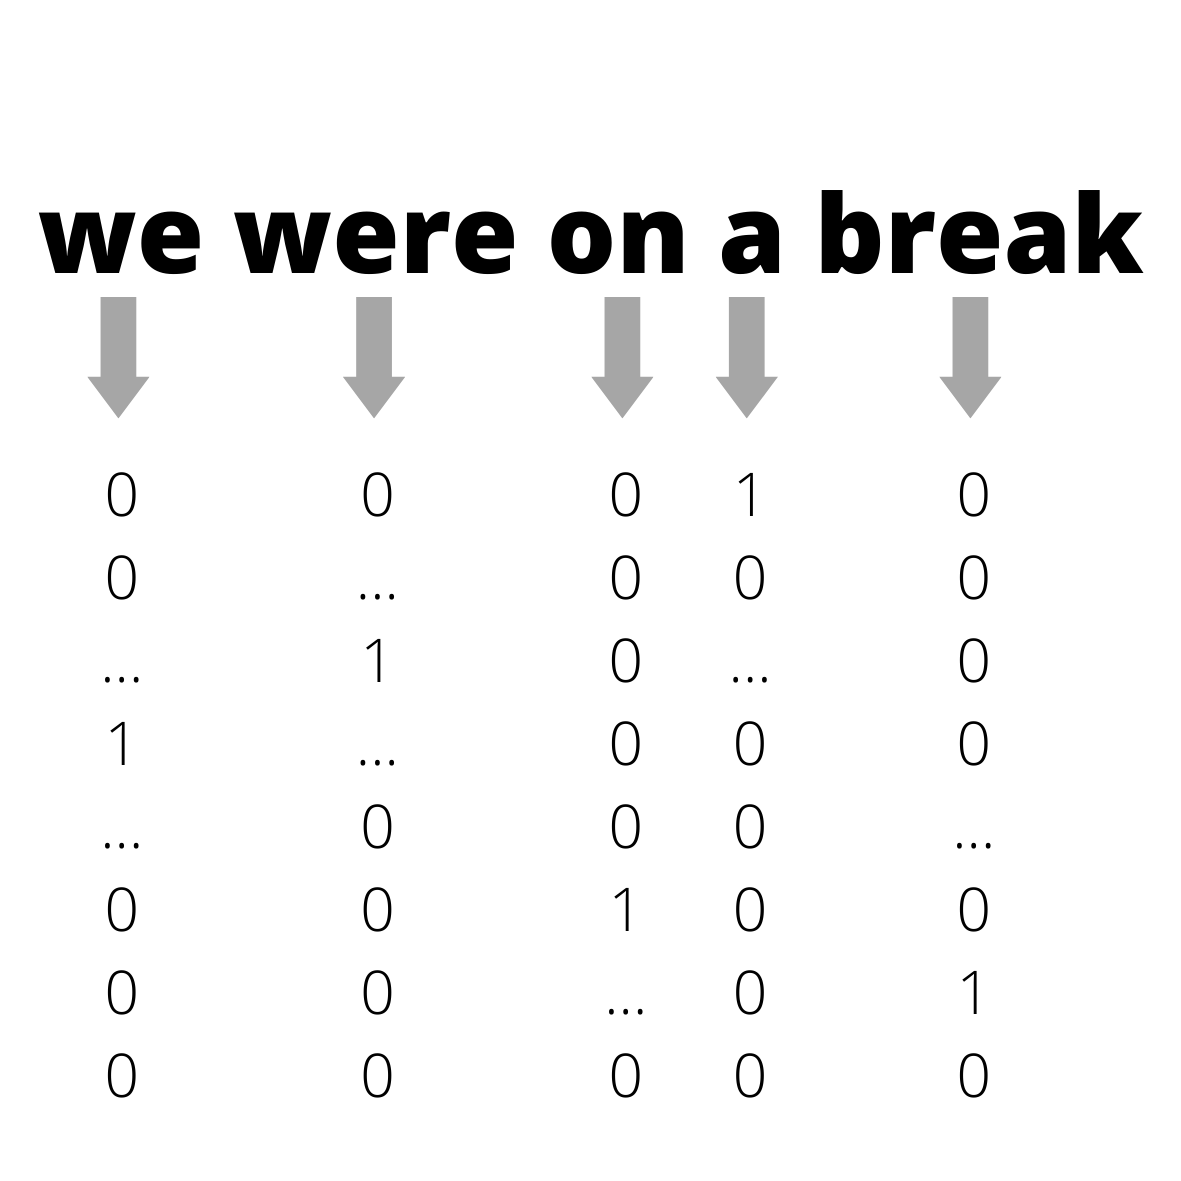
\includegraphics[width = 5cm]{img/one_hot_encoding.png}}
        \only <2> {
            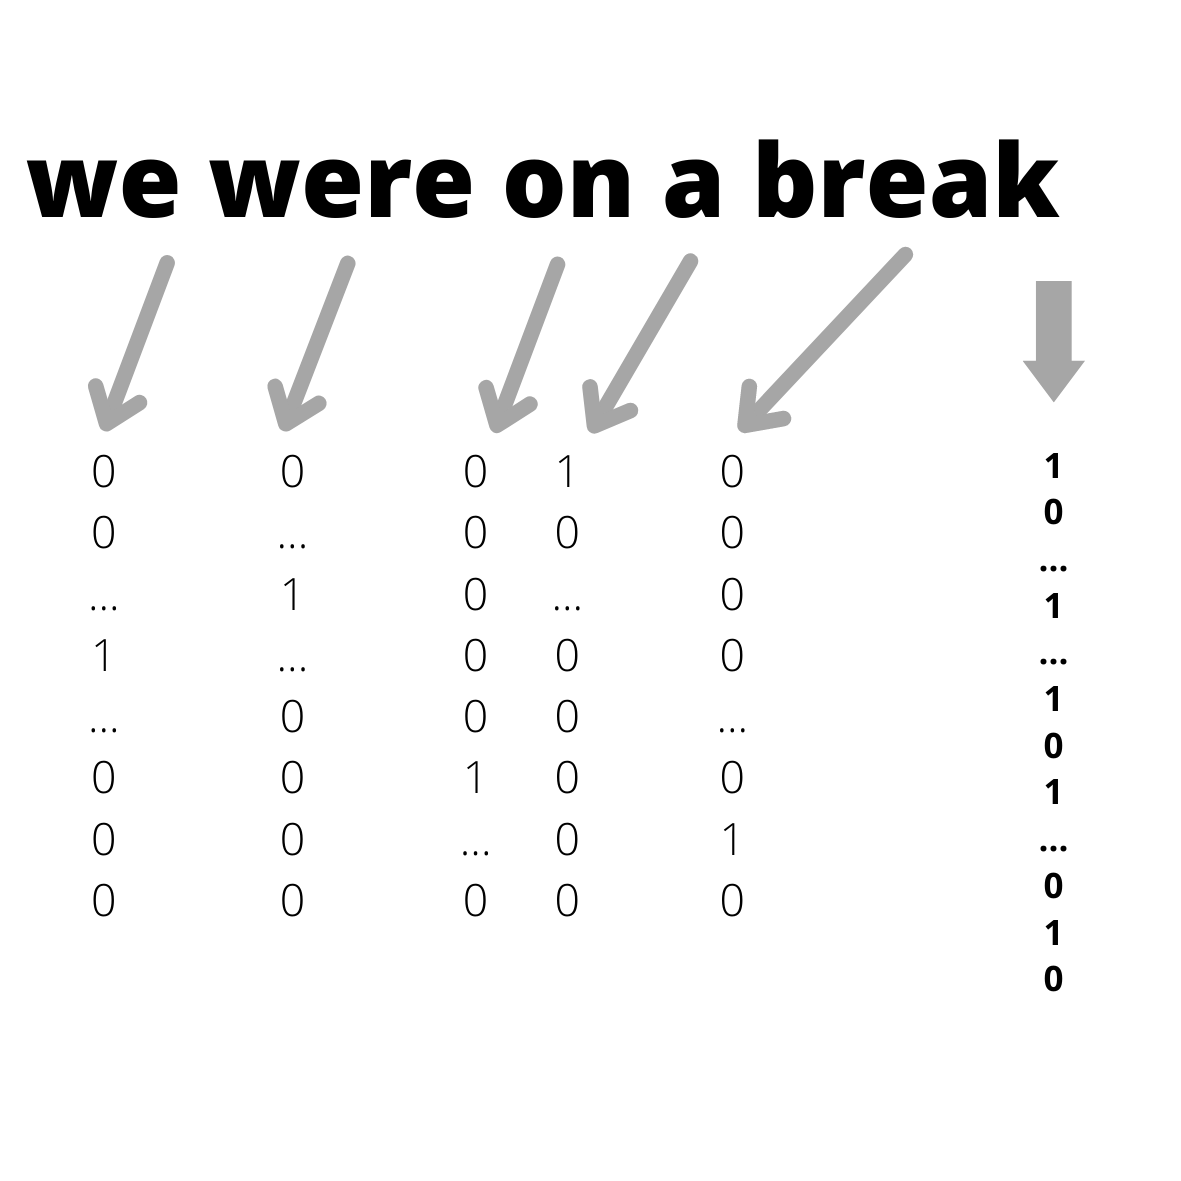
\includegraphics[width = 5cm]{img/BOW.png}}
    \end{column}
\end{columns}
\end{frame}


\subsection{Language Models}
\begin{frame}
    \frametitle{Table of contents}
    \tableofcontents[currentsection]
\end{frame}

\begin{frame}{What are Language Models?}
    In the previous section we named some applications of NLP such as Machine Translation, Natural Language Generation, Sentiment Analysis, etc. However, with Word Embeddings, we have only taken the first step. \vspace{0.2cm}\\
    The aforementioned tasks need \textbf{representations of sentences or documents}, therefore the use of Language Models (\textbf{LM}). Formally, a LM consists of assigning a probability to a sequence of words $\{w_1,\dots,w_n\}$. Moreover, this is equivalent to the problem of \textbf{finding a missing word in the sequence}\footnote{\url{https://towardsdatascience.com/language-models-1a08779b8e12}}:
    $$ p(w_i|w_1,\dots,w_n) = \displaymode \frac{p(w_1,\dots,w_i)}{p(w_1,\dots,w_n)} $$
    In practice, we will use Language Modelling to train representations rather than directly using the probabilities.
\end{frame}


\begin{frame}{Local Normalisation}
    % \textit{Transformers} es un ejemplo de modelo auto-regresivo profundo, i.e., modelos generativos secuenciales que predicen valores futuros de una sucesión dado su pasado. Más precisamente, los modelos que nos conciernen son aquellos que modelan las probabilidades de la secuencia de manera siguiente:
    Some LMs we will study correspond to deep auto-regressive models, i.e., generative models that predict future values of a sequence given its past. Formally, we are concerned with thode modelling probabilities in the following way:
    % $$ p_{ML}(x_{p+1},\dots,x_T|x_1,\dots,x_p) = \prod_{i=p+1}^T p(x_i|x_1,\dots,x_{i-1}) = \prod_{i=p+1}^T \frac{s(x_1,\dots,x_p,\dots,x_{i})}{\sum_{y\in V}s(x_1,\dots,x_p,\dots,x_{i-1},y)}\,,$$
    \begin{alignat*}{2}
    p_{ML}(x_{p+1},\dots,x_T|x_1,\dots,x_p) & = \prod_{i=p+1}^T p(x_i|x_1,\dots,x_{i-1}) \\
    & = \prod_{i=p+1}^T \frac{s(x_1,\dots,x_p,\dots,x_{i})}{\sum_{y\in V}s(x_1,\dots,x_p,\dots,x_{i-1},y)}\,,
    \end{alignat*}
    where $s(x_1,\dots,x_p,\dots,x_{i-1},y)$ is a score of a token $y$ given the input $x_1,\dots,x_p$ and the prediction history $x_{p+1},\dots,x_{i-1}$. This is called ``local normalisation''. This way, models are capable of producing language in a sequential way.
    % donde $s(x_1,\dots,x_p,\dots,x_{i-1},y)$ es un el score del token $y$ dado el input $x_1,\dots,x_p$ y el historial de predicción $x_{p+1},\dots,x_{i-1}$. A esto se le llama ``normalización local''. De esta manera, los modelos de lenguaje son capaces de producir lenguaje de manera secuencial (token por token), además de ser útiles para otras tareas usando transfer-learning. Los MLs se entrenan en grandes corpuses de texto al maximizar la verosimilitud.
\end{frame}


% \subsection{Neural probabilistic LMs}
\begin{frame}{Neural probabilistic LMs}
    \vspace{0.3cm}\\
    In Neural LM we combine vectors using \textbf{neural networks}. Literally from Bengio et al. 2003:
    \begin{enumerate}
        \item associate with each word in the vocabulary a distributed word feature vector (a real valued vector), 
        \item express the joint probability function of word sequences in terms of the feature vectors of these words in the sequence, and 
        \item learn simultaneously the word feature vectors and the parameters of that probability function.
    \end{enumerate}
\end{frame}


\begin{frame}{Neural probabilistic LMs}
\vspace{0.3cm}\\
\begin{columns}[onlytextwidth]
    \begin{column}{0.50\textwidth}
    Results depend heavily on the architecture to use.
    The simplest option is using a simple \textbf{Multi-layer perceptron} as in Bengio et al.. % \cite{bengio}. %explain further
    However, this is arguably not the best option to encode language.
    \vspace{0.2cm}\\ We will go through two more options that are widely used today:
    \begin{itemize}
        \item Recurrent Neural Networks (RNN)
        \item Transformers
    \end{itemize}
    \end{column}
    \begin{column}{0.50\textwidth}
        \centering
        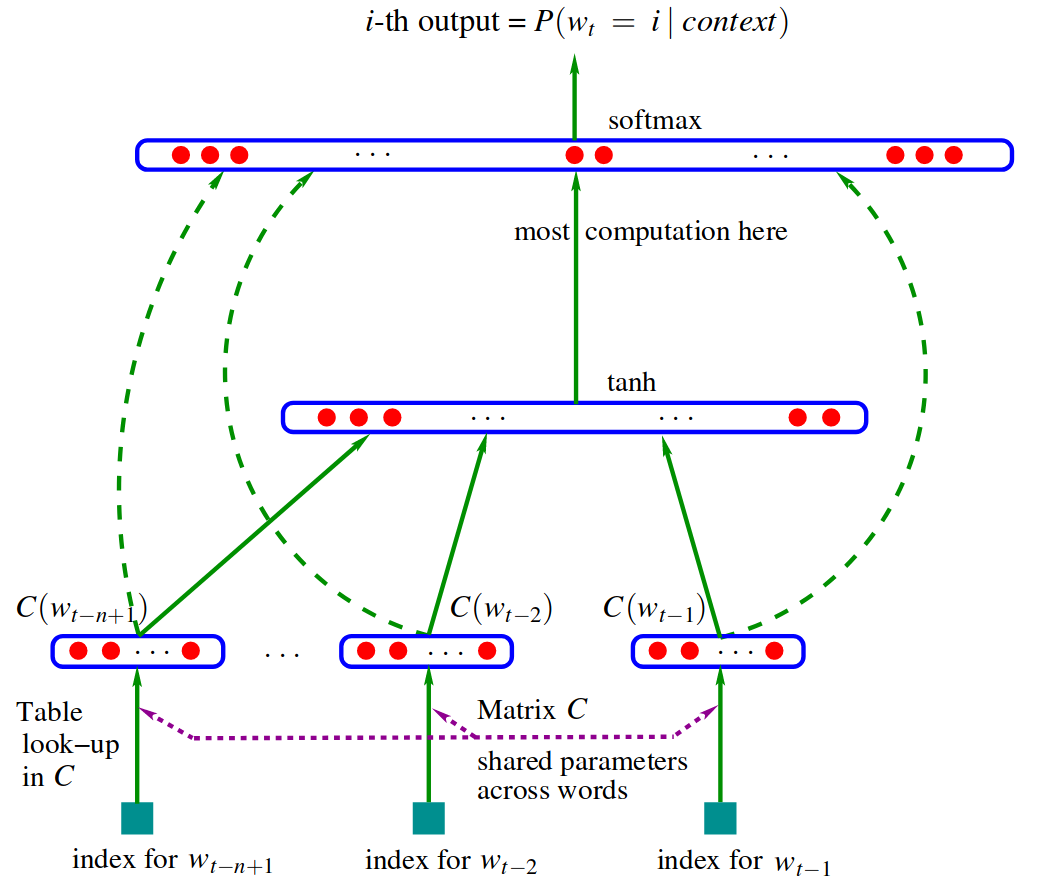
\includegraphics[width = 6cm]{img/bengio.png}
    \end{column}
\end{columns}
\end{frame}


\iffalse
\subsection{n-gram language models}
% https://en.wikipedia.org/wiki/Language_model#Notable_language_models
% https://web.stanford.edu/~jurafsky/slp3/3.pdf
% http://www.cs.columbia.edu/~mcollins/cs4705-spring2019/slides/lmslides.pdf

% difference between transformer LMs
% https://neptune.ai/blog/unmasking-bert-transformer-model-performance
\fi


\subsection{Learning objectives and perplexity}
\begin{frame}{Learning Objectives}
    Back in 2003, Bengio et al. 2003 introduced on the first \textbf{Neural Language Models}. % \cite{bengio}. 
    Neural LMs are characterised by making use of word embeddings. But, how do we assign a probability distribution to documents or sentences? We'll discuss three methods:
    \begin{itemize}
        \item \textbf{Next word prediction (NWP)}
        \only <3,4,5,6,7>{
        \item \textbf{Masked Language Model (MLM)}}
        \only <6,7>{
        \item \textbf{Next sentence prediction (NSP)}}
    \end{itemize}
\only <1>{
% \begin{textblock}{0.15}(0.07, 0.6)
\begin{figure}
    \centering
    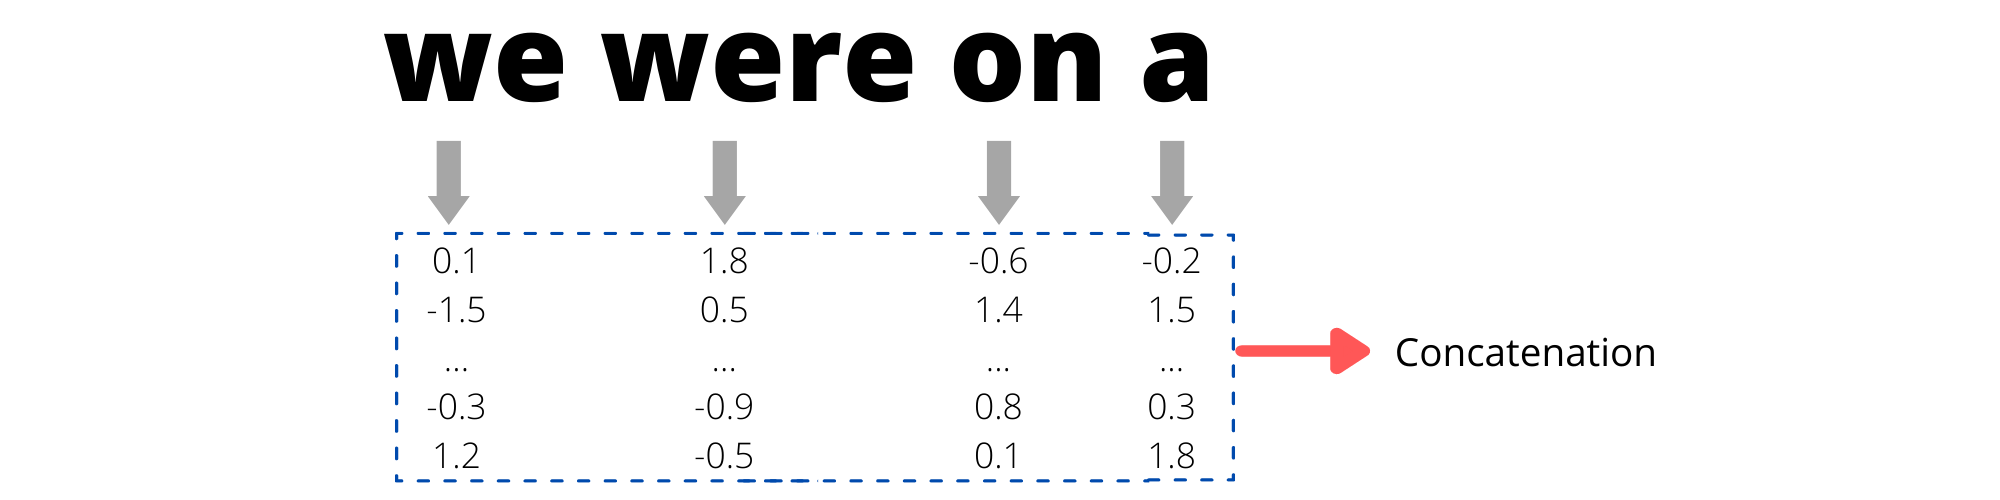
\includegraphics[width = 11cm]{img/NWP1.png}
    % \caption{Caption}
    % \label{fig:enter-label}
\end{figure}
% \end{textblock}
}
\only <2>{
\centering
    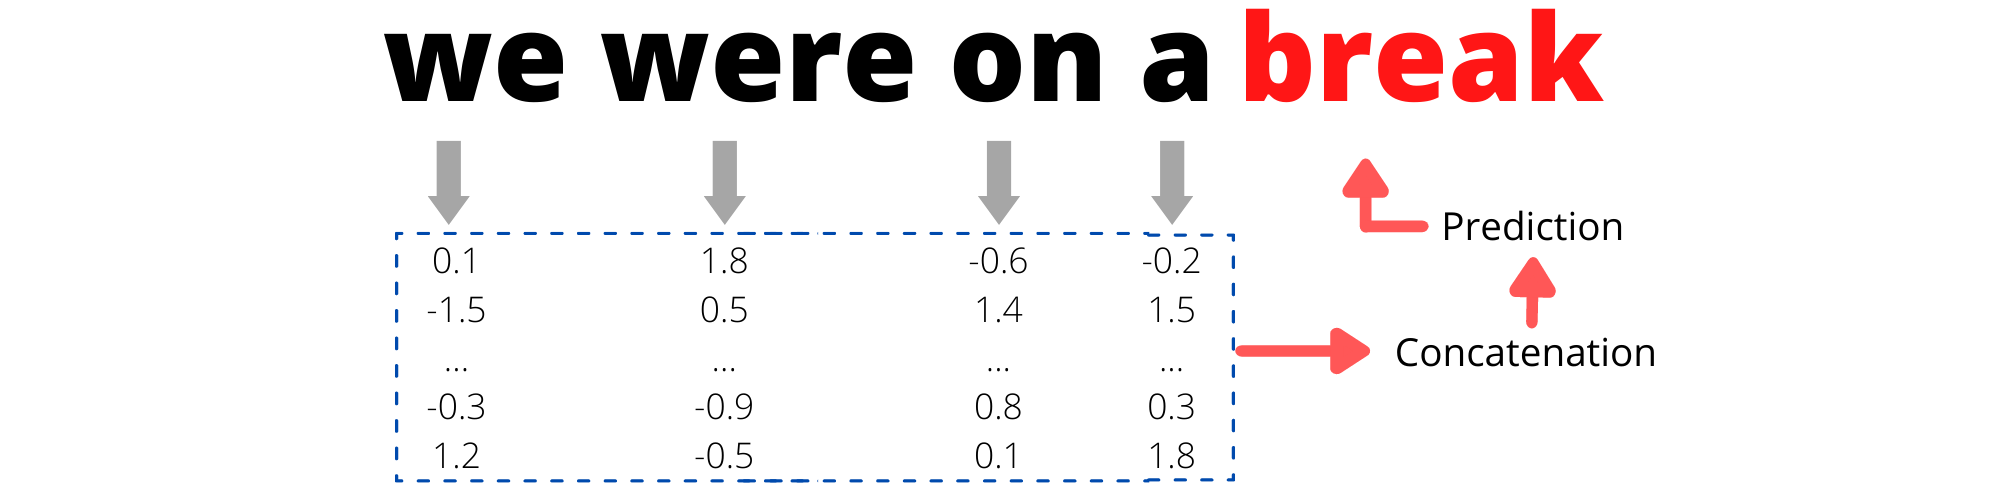
\includegraphics[width = 11cm]{img/NWP2.png}
}
\only <6>{\centering
    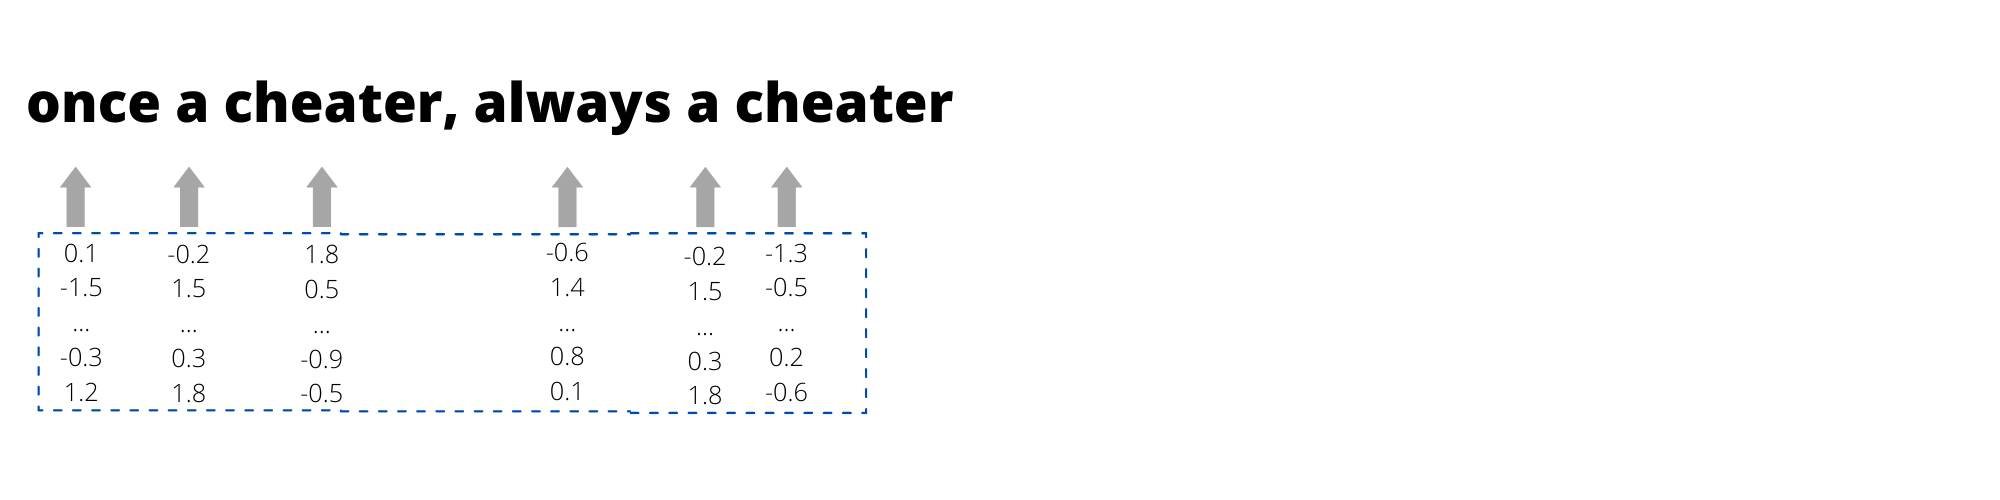
\includegraphics[width = 11cm]{img/NSP1.png}
}
\only <7>{\centering
    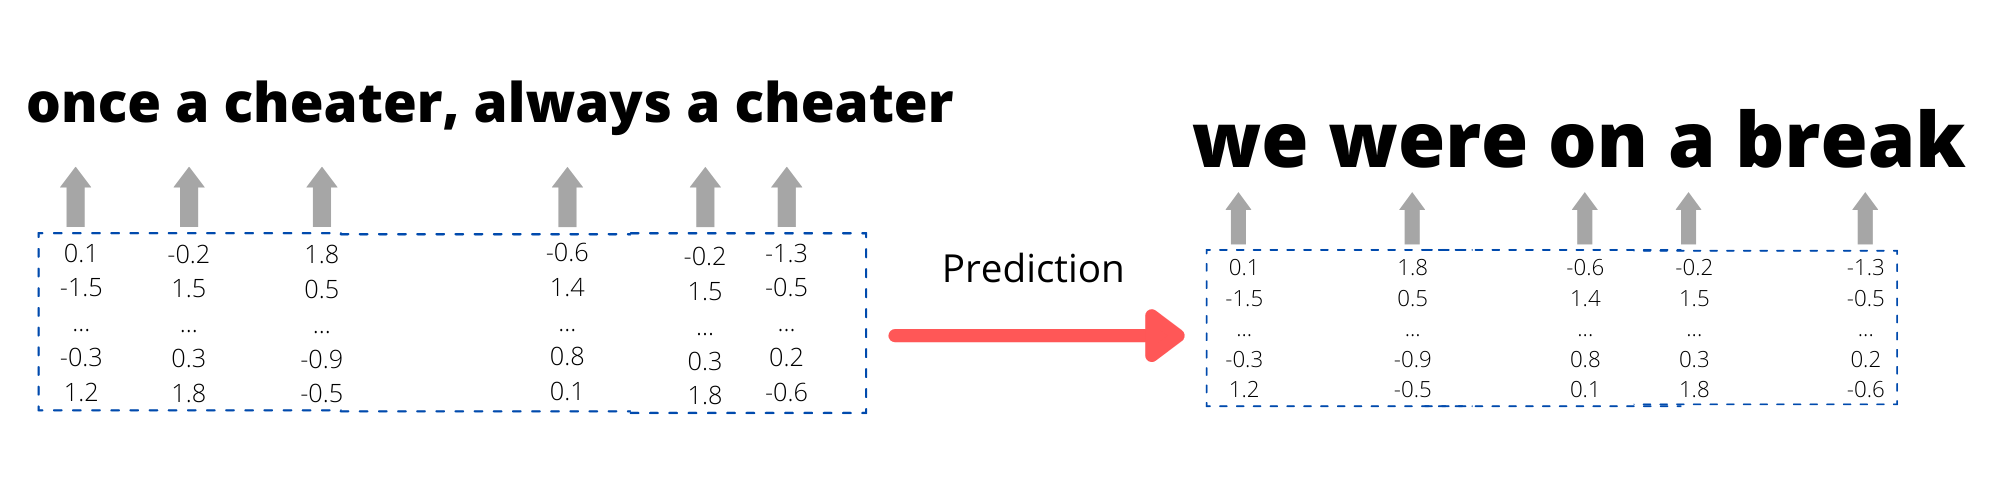
\includegraphics[width = 11cm]{img/NSP2.png}}
\only <3>{\centering
    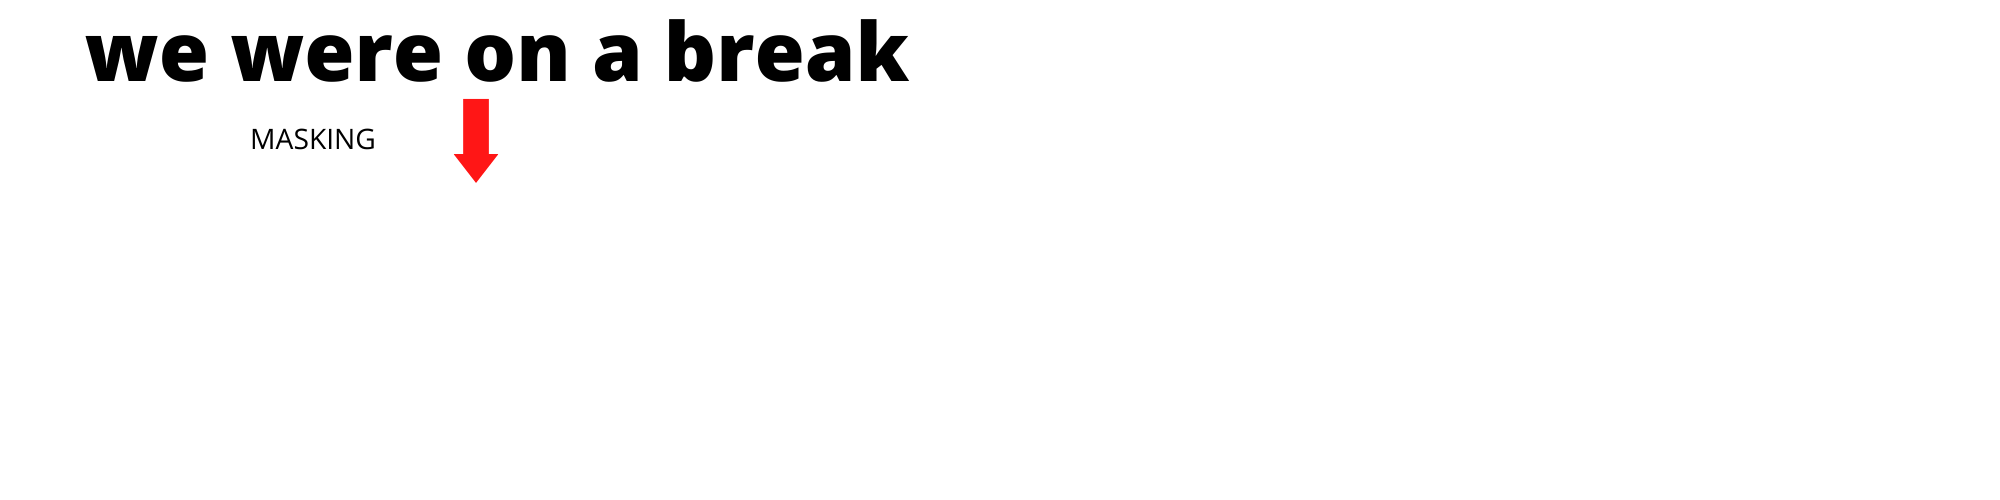
\includegraphics[width = 12cm]{img/MLM.png}}
\only <4>{\centering
    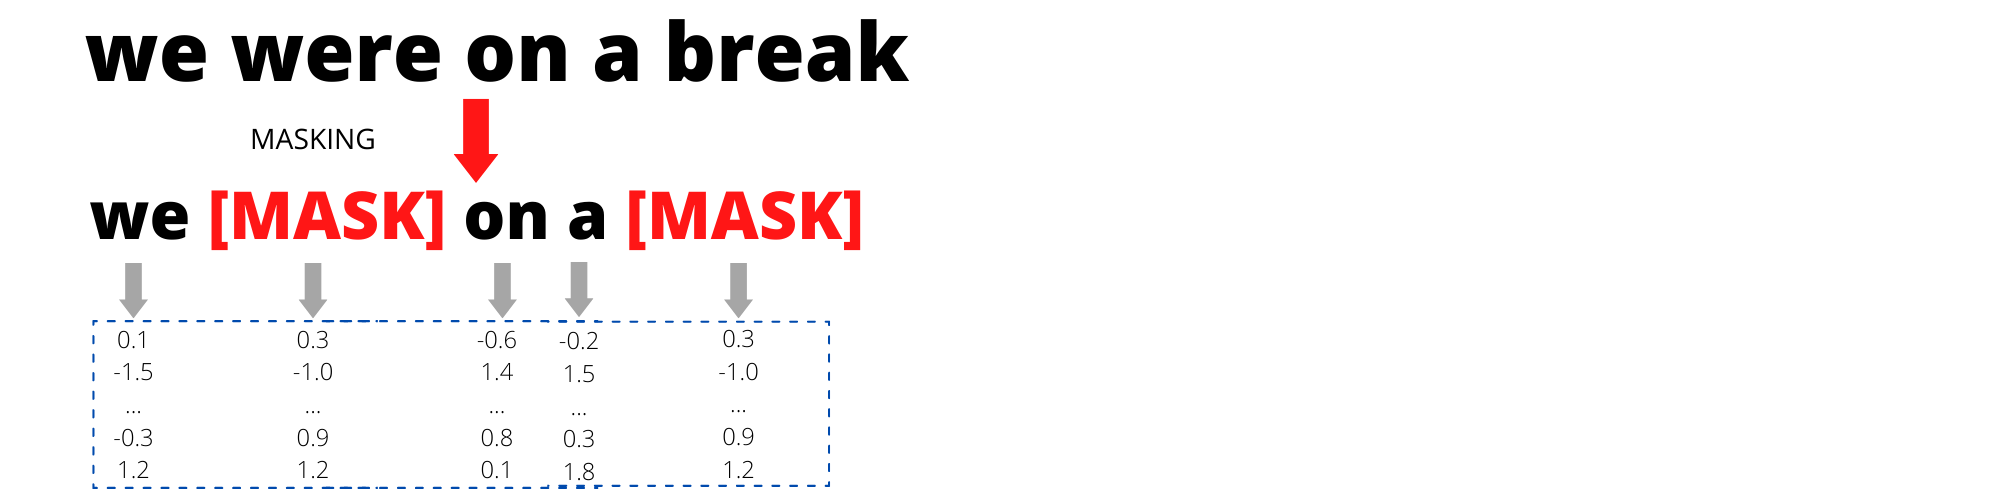
\includegraphics[width = 12cm]{img/MLM2.png}}
\only <5>{\centering
    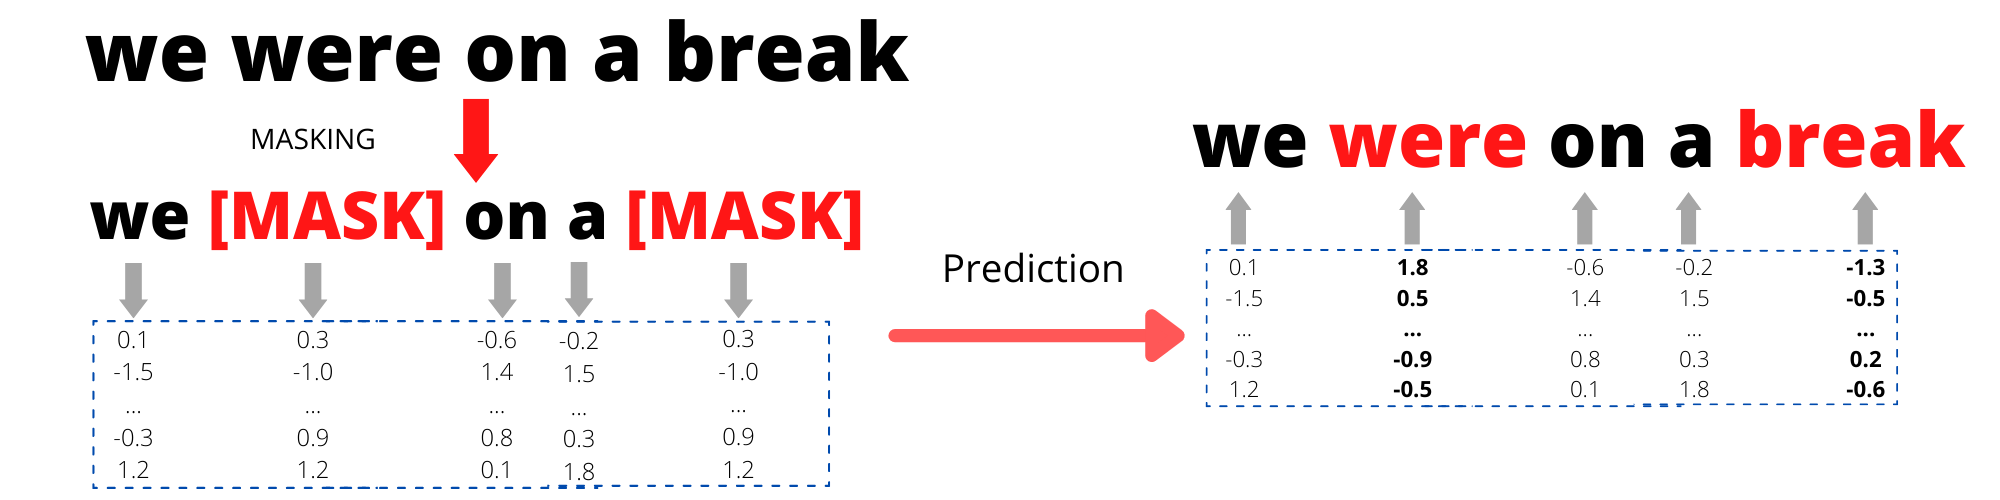
\includegraphics[width = 12cm]{img/MLM3.png}}
\end{frame}


\begin{frame}{Evaluation: Perplexity}
    \vspace{0.3cm}\\
    \textbf{Perplexity} (PPL) is a widely used evaluation metric for language models, specially when the target task is text generation. It is defined as 
    $$ 2^{-\frac{1}{T-p}\sum^T_{i=p+1}\log_2p(x_i|x_{i-1},\dots,x_1)} \,.$$
    It can be interpreted as the mean of the number of tokens for which the model is unsure at each generation step. This is equivalent to the exponentiation of the cross-entropy between the data and model predictions\footnote{\url{https://huggingface.co/docs/transformers/perplexity}}.
    % PPL is sometimes defined geometric average of $\frac{1}{p(x_i|x_{i-1},\dots,x_1))}$
    \vspace{0.3cm}\\
    We are often maximising other functions when fitting language models, for instance when using it for other NLP tasks, for which domain specific target metrics exist.
\end{frame}

\begin{frame}{Architectures for Language Modelling}
\vspace{0.3cm}\\
\begin{columns}[onlytextwidth]
    \begin{column}{0.50\textwidth}
    In Neural LM we combine vectors using \textbf{neural networks}. The simplest option is using a simple \textbf{Multi-layer perceptron} as in Bengio et al.. 
 % \cite{bengio}. %explain further
    However, this is arguably not the best option to encode language.
    \vspace{0.2cm}\\ We will go through two more options that are widely used today:
    \begin{itemize}
        \item Recurrent Neural Networks (RNN)
        \item Transformers
    \end{itemize}
    \end{column}
    \begin{column}{0.50\textwidth}
        \centering
        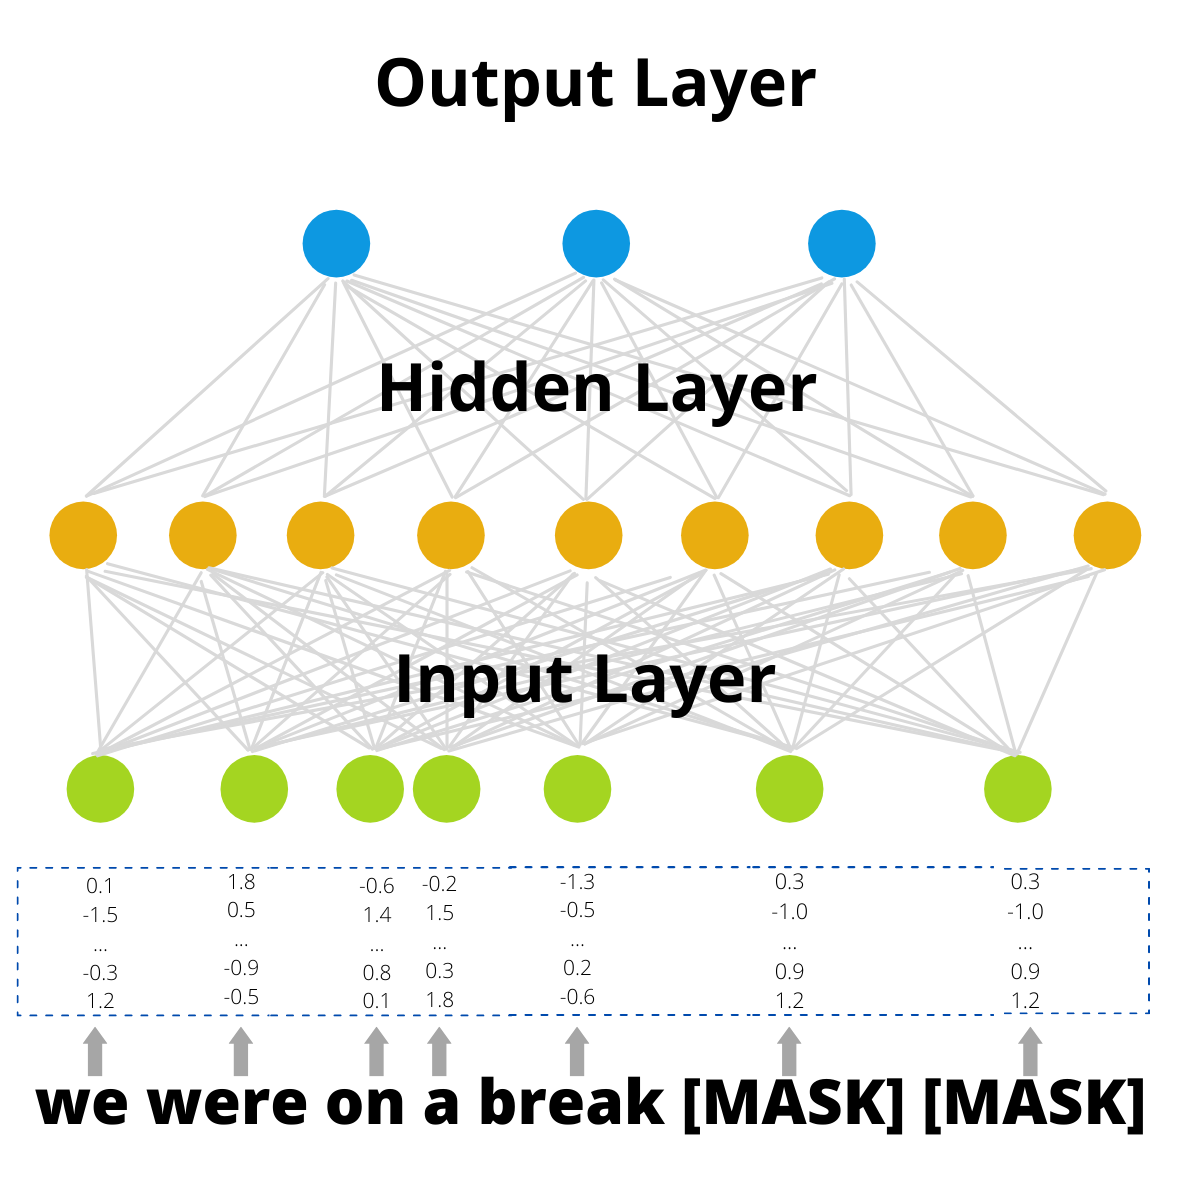
\includegraphics[width = 6cm]{img/MLP.png}
    \end{column}
\end{columns}
\end{frame}


\section{The Transformer architecture}
% \subsection{Attention}
\begin{frame}
    \frametitle{Table of contents}
    \tableofcontents[currentsection]
\end{frame}

\subsection{Recurrent Neural Networks}

% \subsection{Vanilla RNN}

\begin{frame}{Recurrent Neural Networks}
%\vspace{0.3cm}\\
    RNNs are an ideal solution to deal with sequences of unknown length. In its simple version (\textbf{Vanilla RNN}) we simply apply a neural network to generate an \textbf{output} and a \tetxbf{hidden state} to every member of the sequence.
\centering
\only <1>{
% \begin{textblock}{0.15}(0.07, 0.42)
        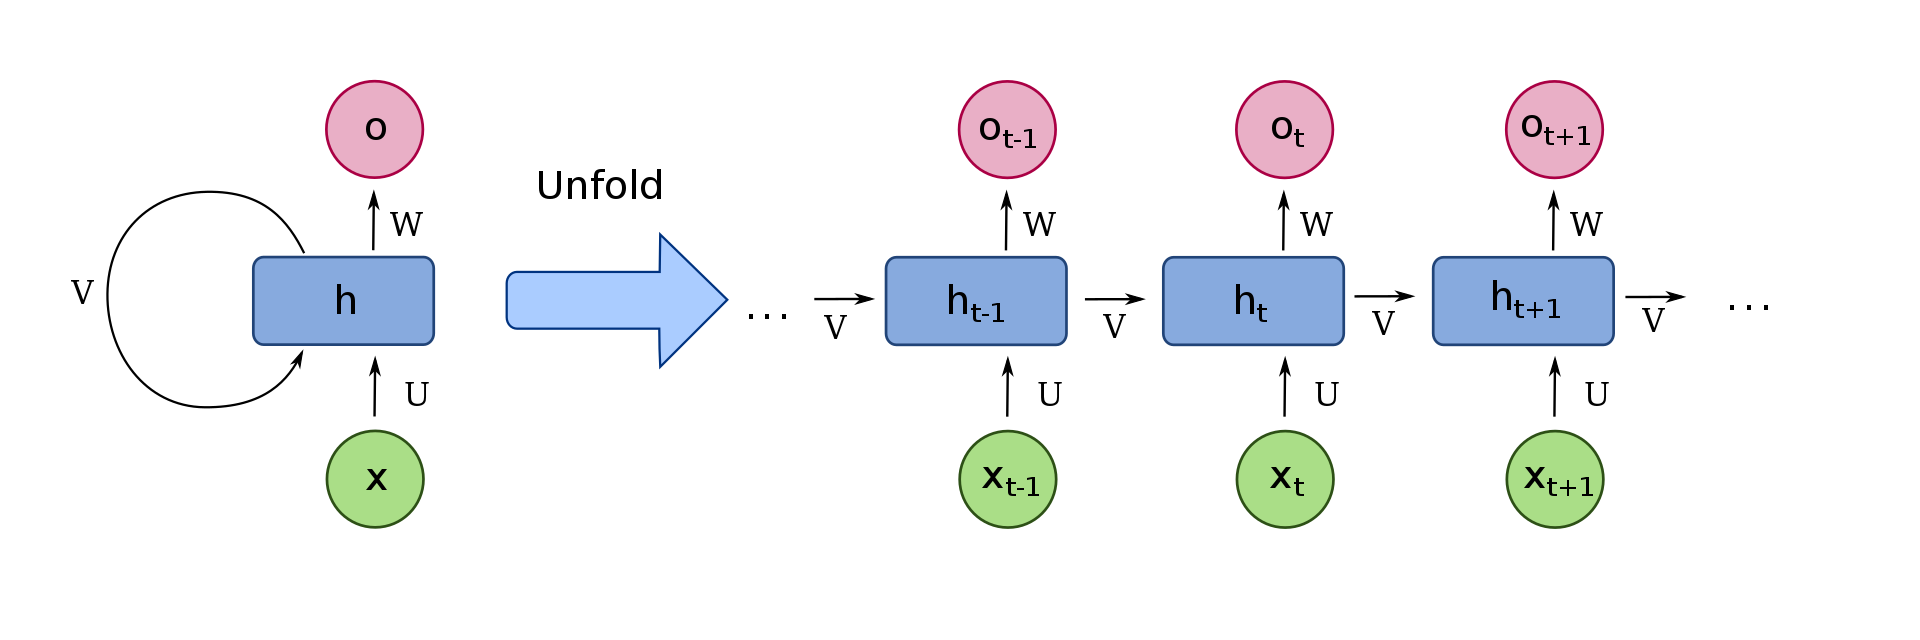
\includegraphics[width = 11cm]{img/rnn.png}
% \end{textblock}
}
\only <2>{
% \begin{textblock}{0.15}(0.07, 0.42)
        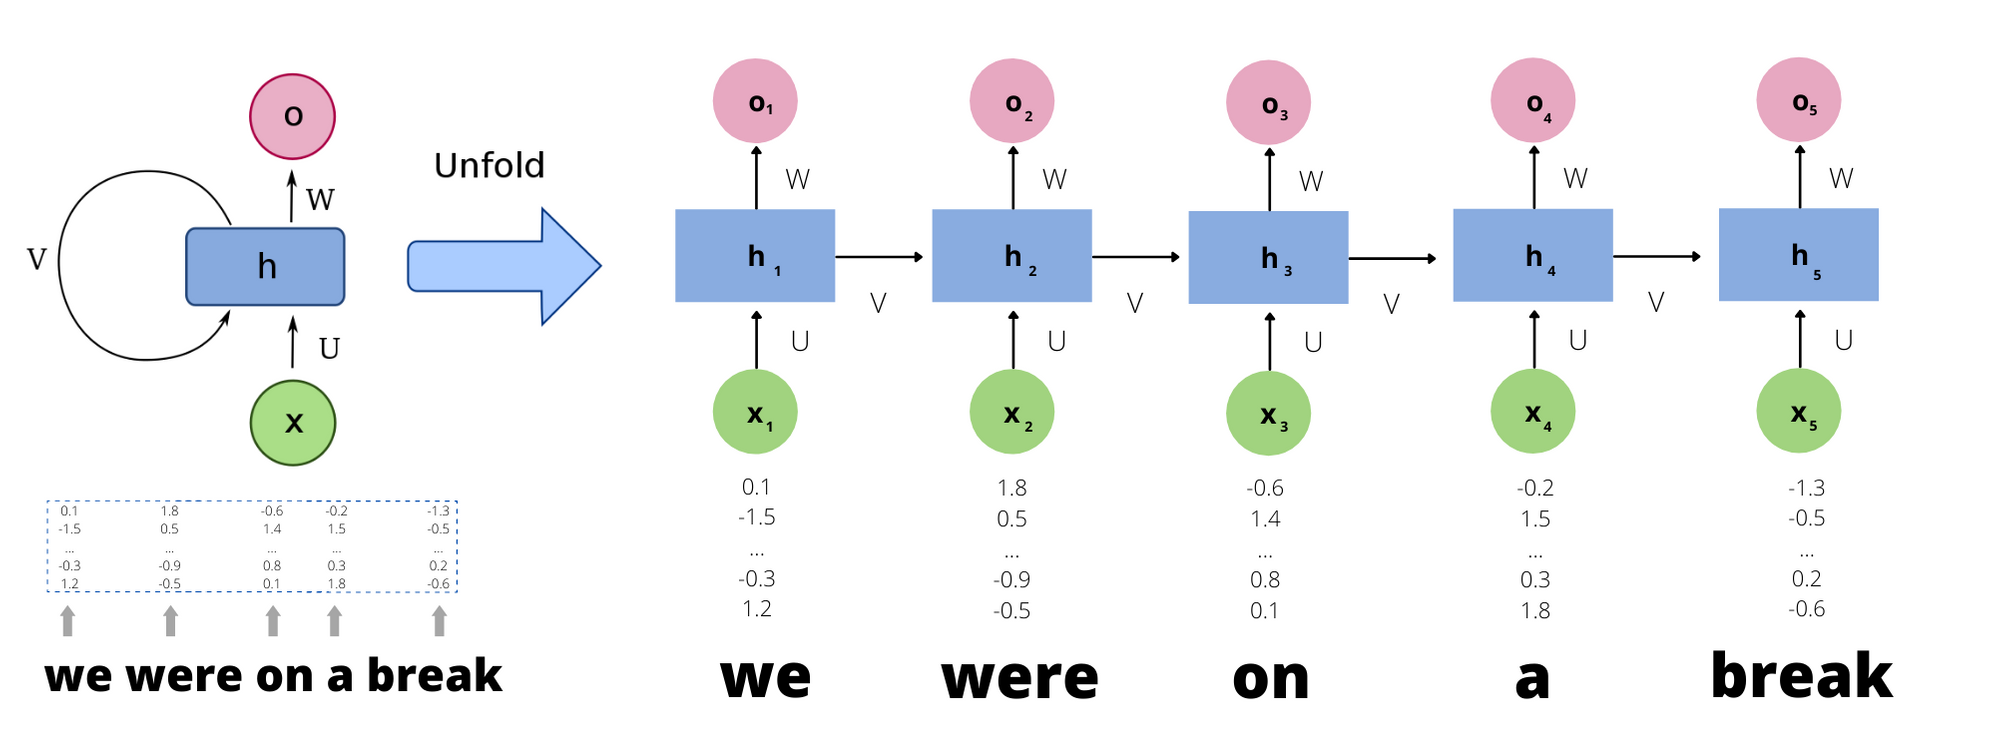
\includegraphics[width = 11cm]{img/rnn_example.png}
% \end{textblock}
}
    \vspace{4.3cm}\\ For any given word, we apply both the input vector and the previous hidden state.
\end{frame}


% \subsection{RNNs in Practice}
\begin{frame}{Bi-directional LSTM}
\vspace{0.3cm}\\
    RNNs are not perfect: in particular, they suffer from the \textbf{vanishing gradient problem}. This is, when we back-propagate the error to update the weights, we loose information, particularly with long sequences.\\
    In reality, we often apply \textbf{bi-directionality}\only <2> { and we use a more complex architecture instead: the \textbf{Long Short Term Memory Network}}.
\centering
\only <1>{
% \begin{textblock}{0.15}(0.07, 0.45)
        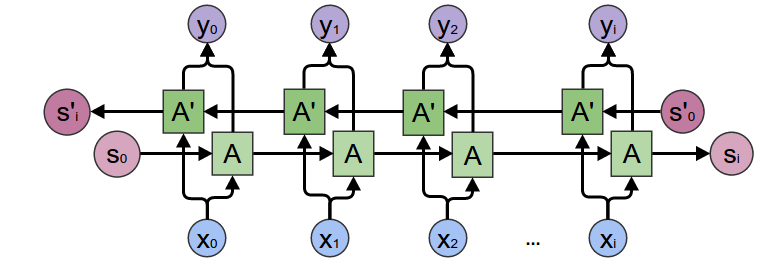
\includegraphics[width = 11cm]{img/bidirectional.png}
% \end{textblock}
}
\only <2>{
% \begin{textblock}{0.15}(0.07, 0.49)
        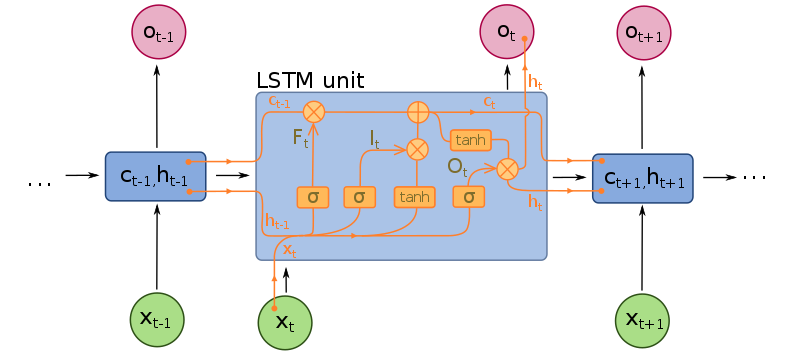
\includegraphics[width = 10cm]{img/lstm.png}
% \end{textblock}
}
\end{frame}



\subsection{Attention}

\begin{frame}{Recurrent Neural Networks}
%\vspace{0.3cm}\\
    RNNs are an ideal solution to deal with sequences of unknown length. In its simple version (\textbf{Vanilla RNN}) we simply apply a neural network to generate an \textbf{output} and a \tetxbf{hidden state} to every member of the sequence.
\only <1>{
\centering
    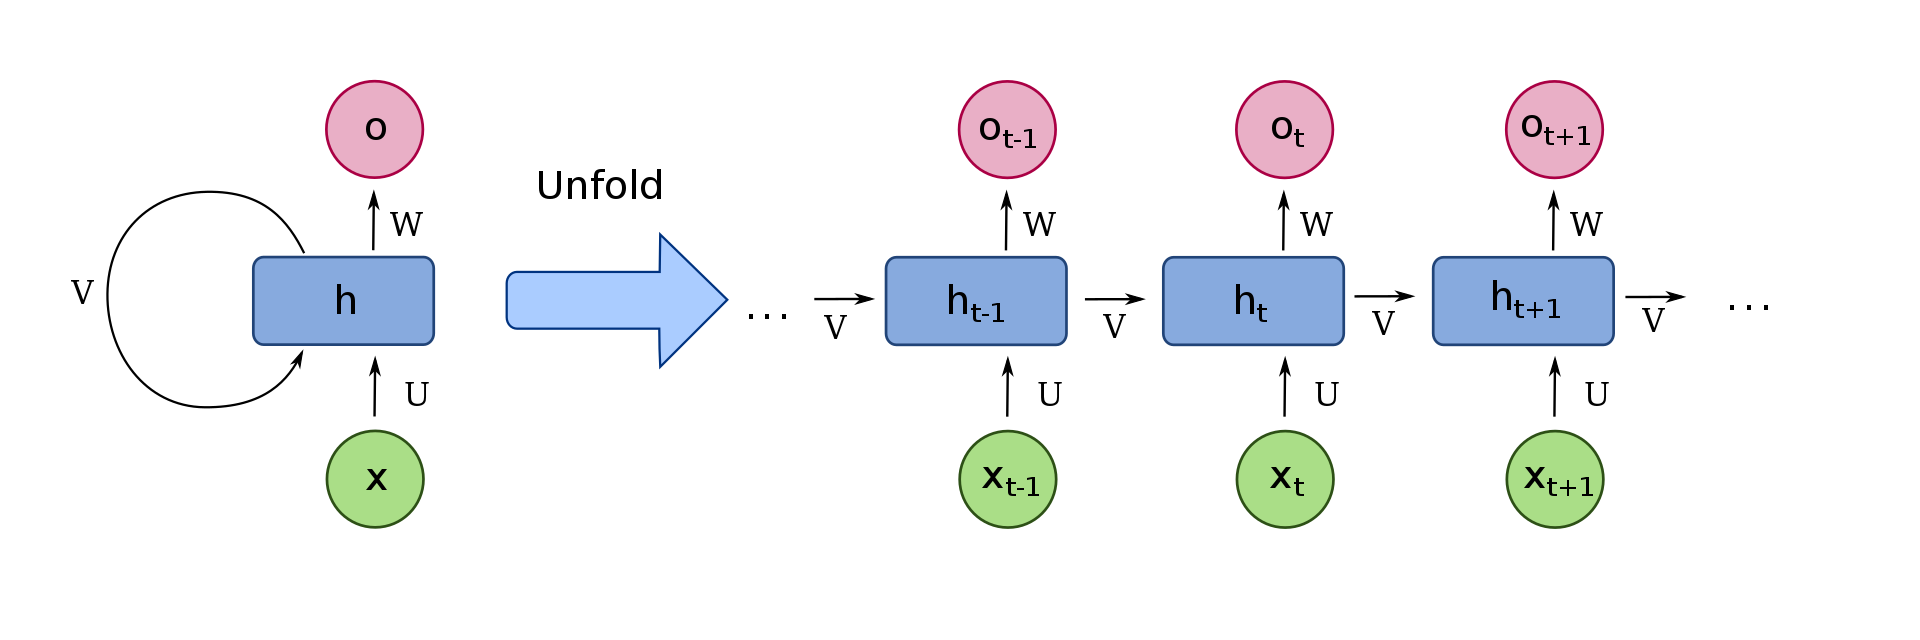
\includegraphics[width = 11cm]{img/rnn.png}}
\only <2>{
\centering
        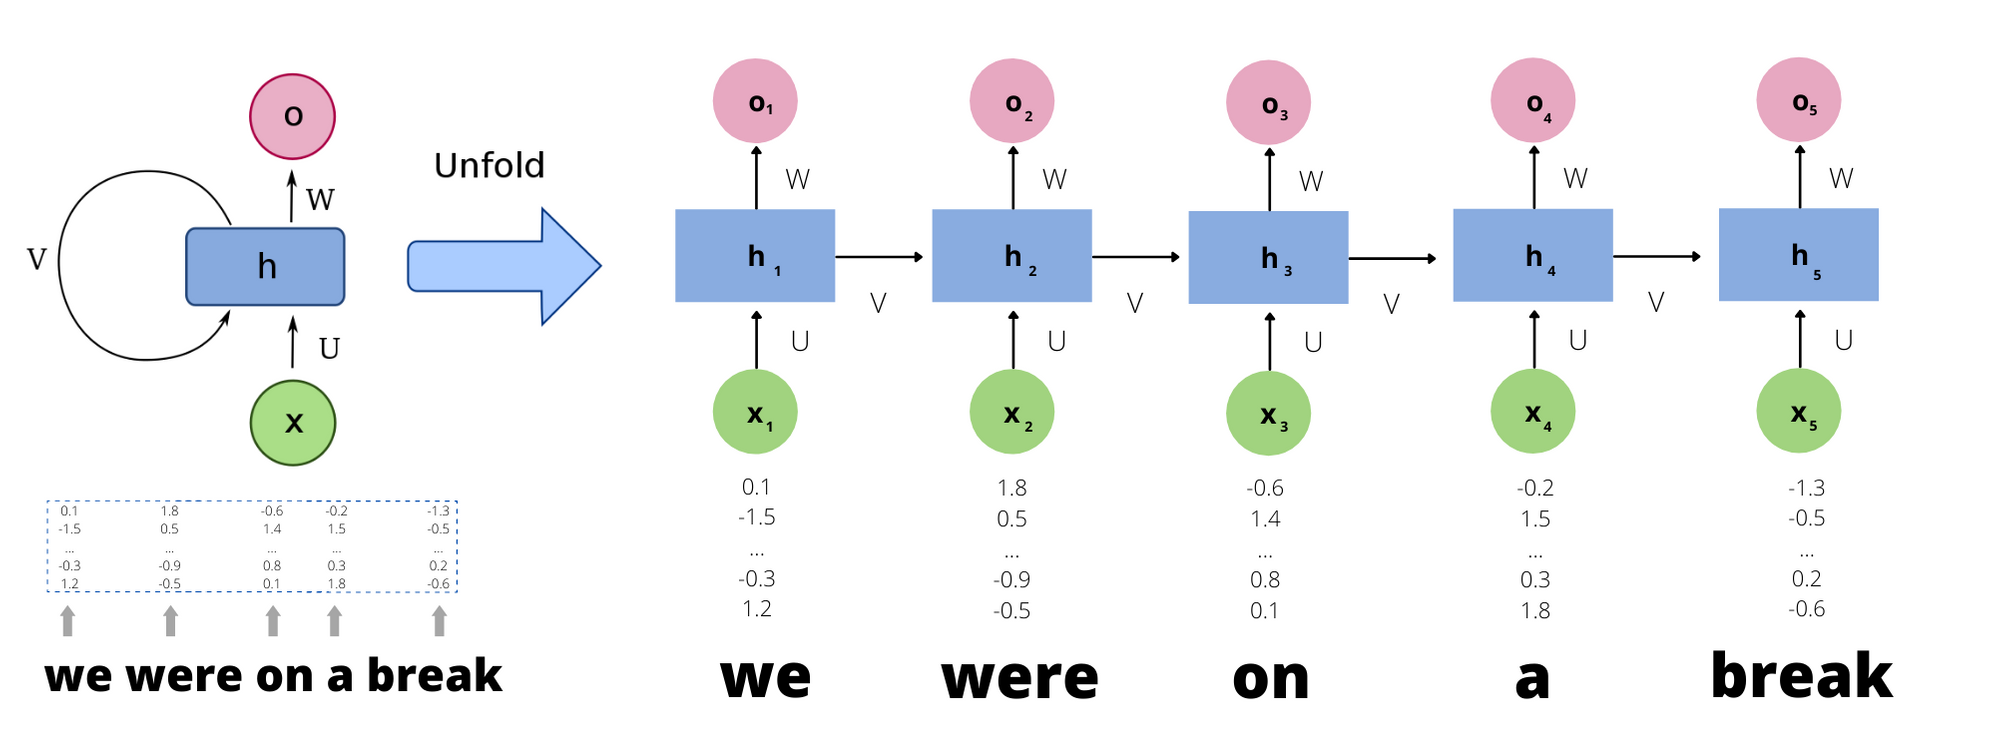
\includegraphics[width = 11cm]{img/rnn_example.png}}
    \vspace{4.5cm}\\ For any given word, we apply both the input vector and the previous hidden state.
\end{frame}

\iffalse
%\subsection{RNNs in Practice}
\begin{frame}{Bi-directional LSTM}
\vspace{0.3cm}\\
    RNNs are not perfect: in particular, they suffer from the \textbf{vanishing gradient problem}. This is, when we back-propagate the error to update the weights, we loose information, particularly with long sequences.\\
    In reality, we often apply \textbf{bi-directionality}\only <2> { and we use a more complex architecture instead: the \textbf{Long Short Term Memory Network}}.
\only <1>{
\centering
    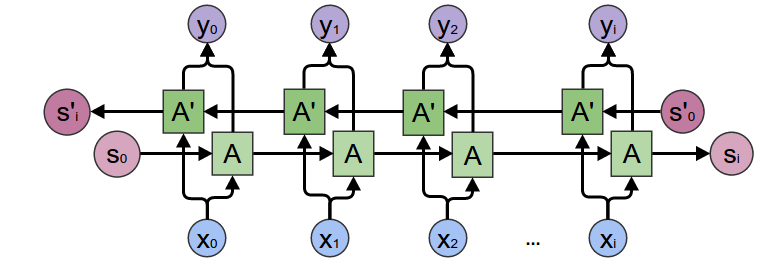
\includegraphics[width = 11cm]{img/bidirectional.png}}
\only <2>{
\centering
    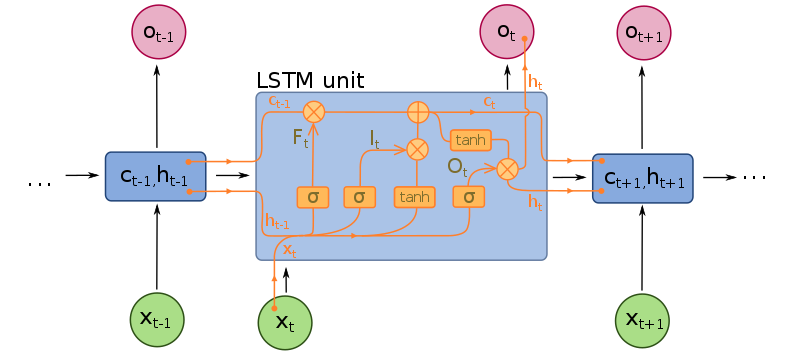
\includegraphics[width = 10cm]{img/lstm.png}}
\end{frame}
\fi

\begin{frame}{RNNs: a Machine Translation example}
\only <1,2,3>{Let's consider an example of \textbf{machine translation}. We will consider an RNN for \textbf{encoding} the input sequence and another one for \textbf{decoding} it into the output sequence.}
\only <4>{A drawback of such a setting is that by encoding the whole sentence in the last output, we are not pushing the decoder to \textbf{focus on the important parts of the input}.
    For example, for computing \textbf{on} in French, we only need to pay attention to the word \textbf{we} in English. }
    \centering
    \only <1>{
% \begin{textblock}{0.15}(0.03, 0.4)
        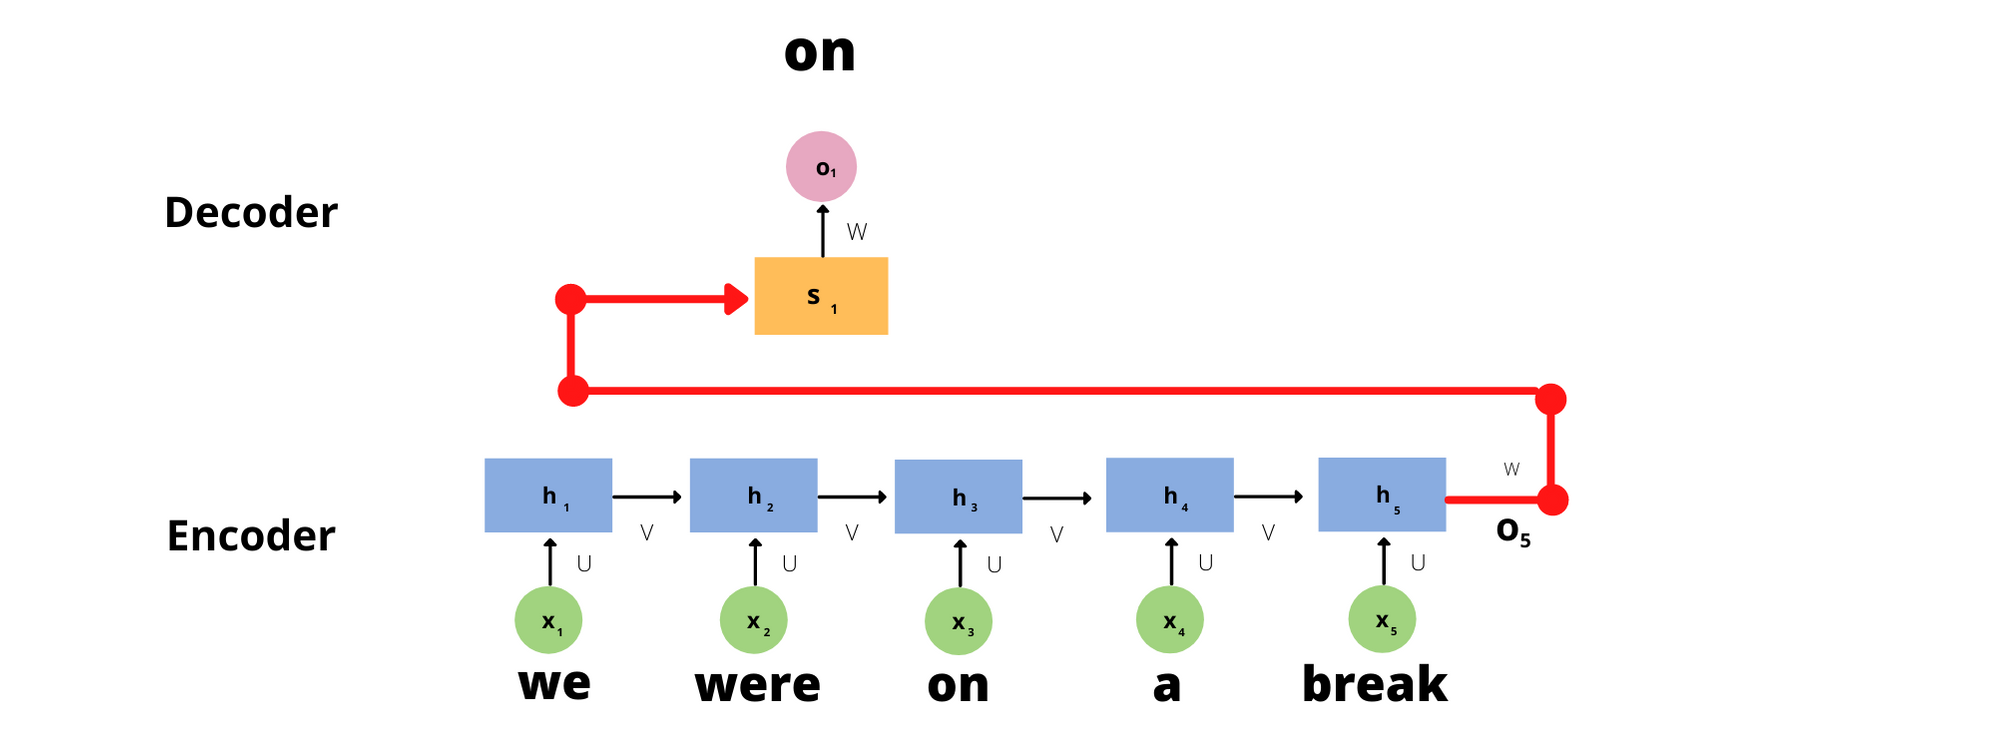
\includegraphics[width = 13cm]{img/RNN_ML1.png}
% \end{textblock}
}
    \only <2>{
% \begin{textblock}{0.15}(0.03, 0.4)
        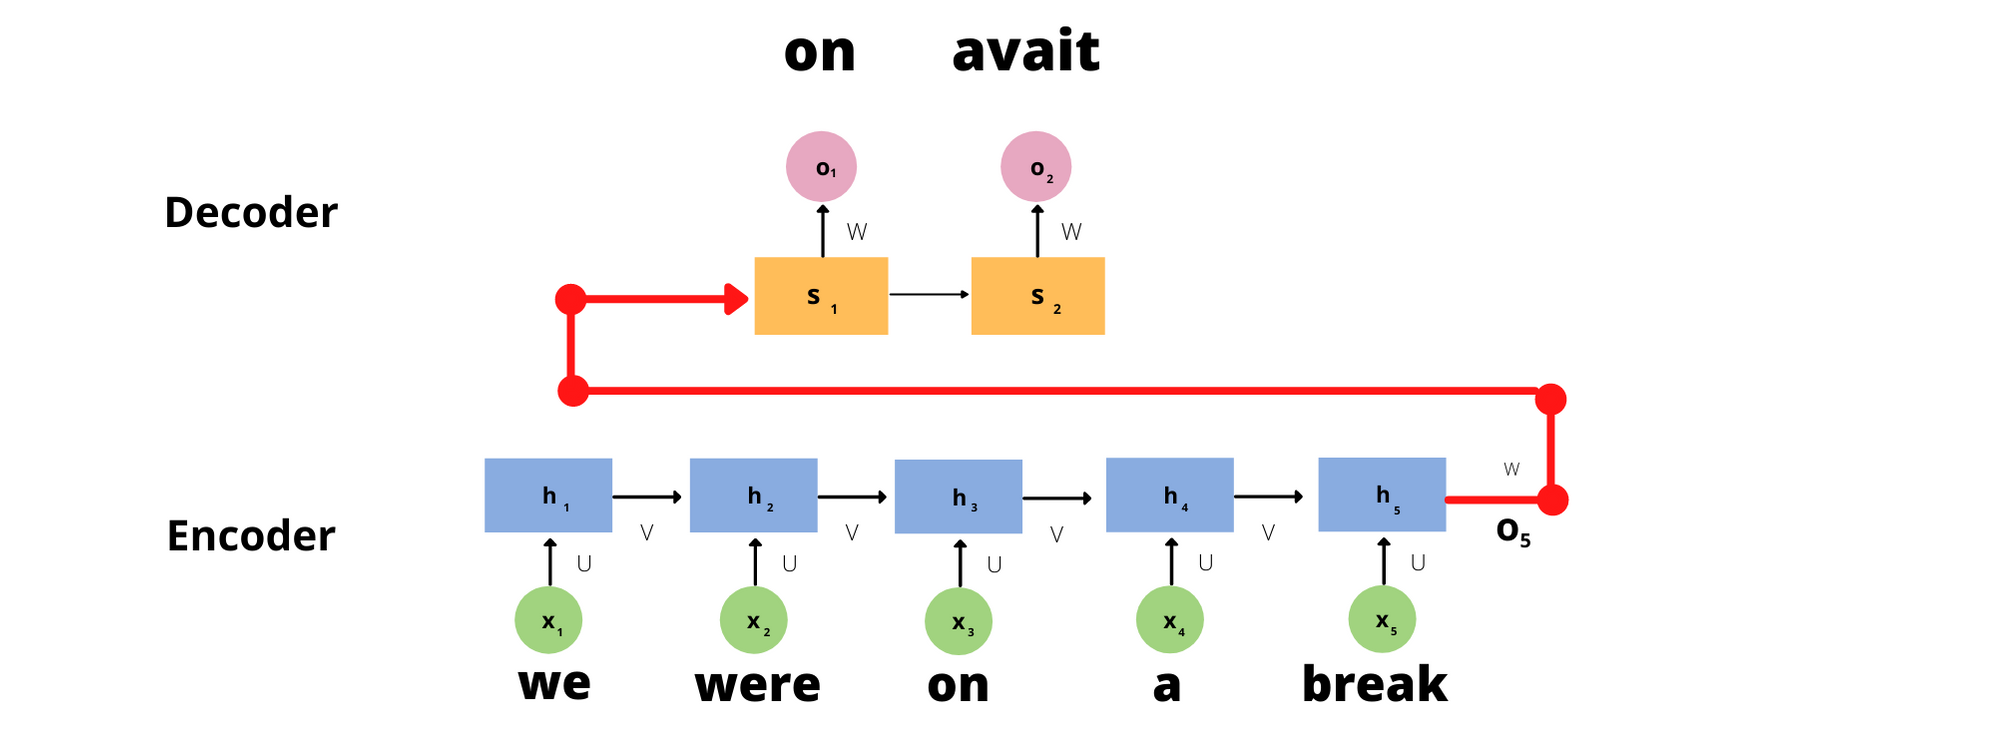
\includegraphics[width = 13cm]{img/RNN_ML2.png}
% \end{textblock}
}
    \only <3>{
% \begin{textblock}{0.15}(0.03, 0.4)
        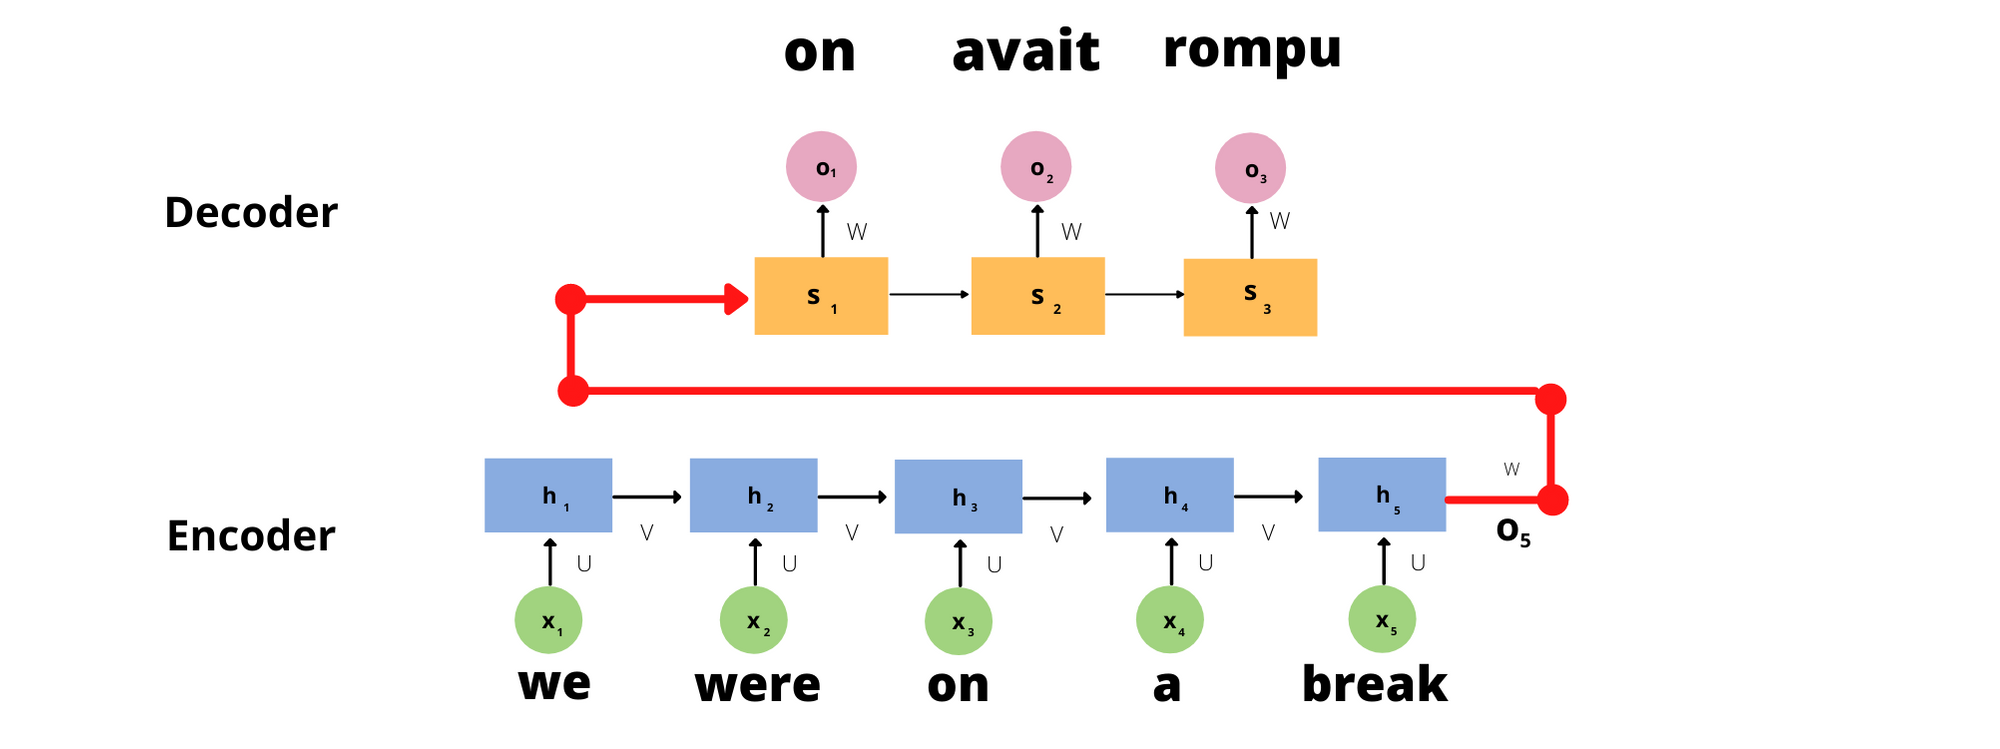
\includegraphics[width = 13cm]{img/RNN_ML3.png}
% \end{textblock}
}
    \only <4>{
% \begin{textblock}{0.15}(0.03, 0.4)
        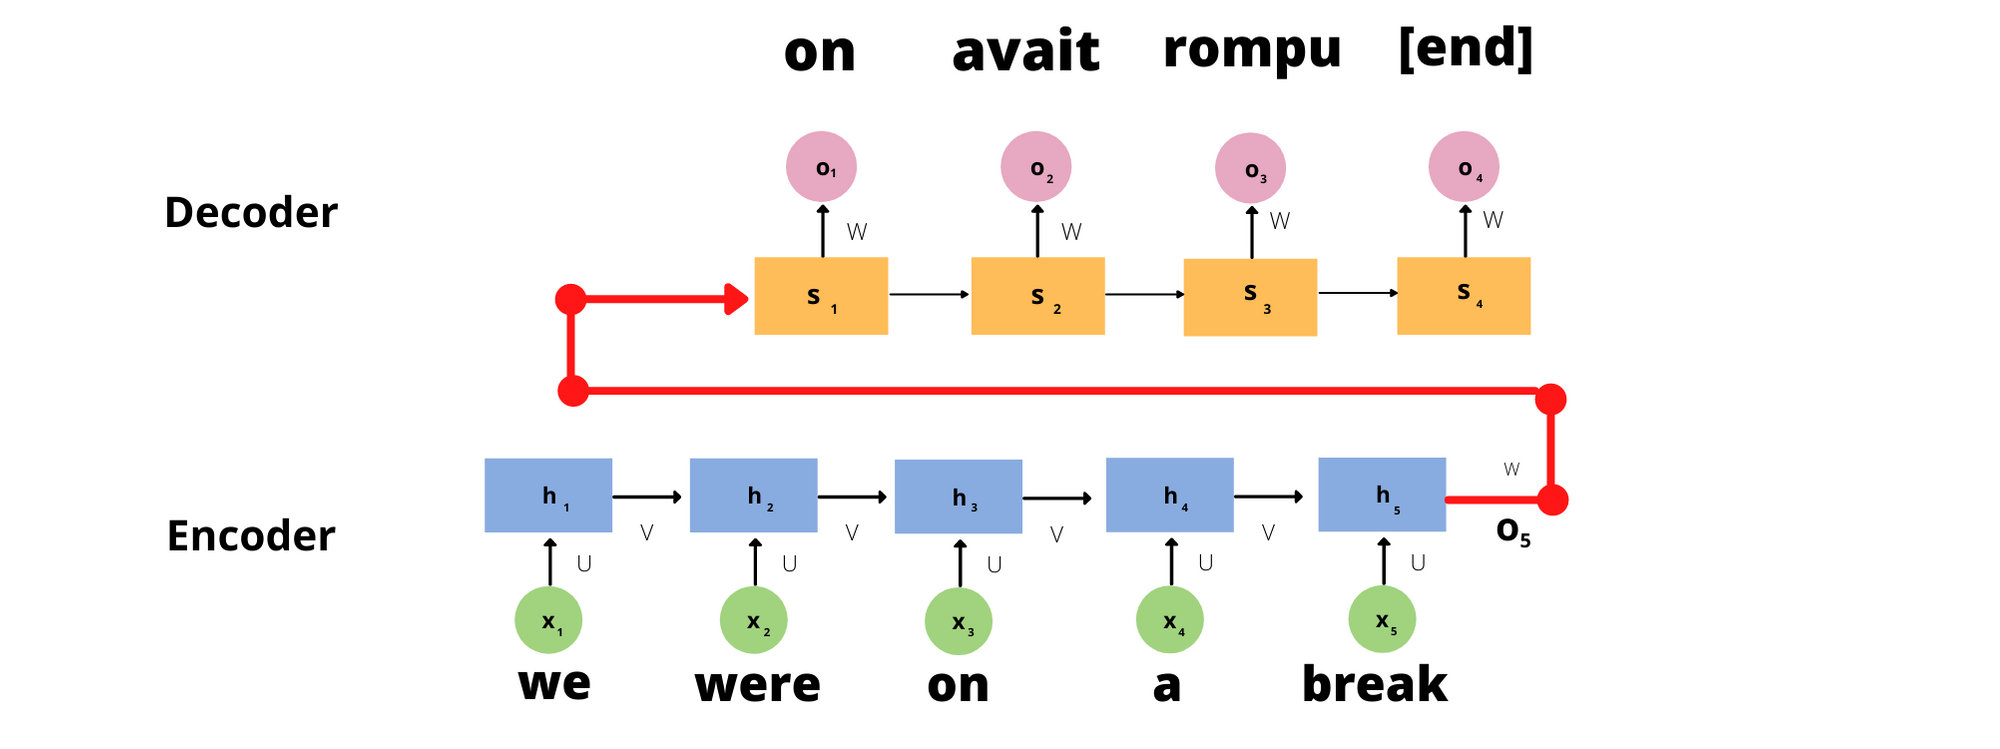
\includegraphics[width = 13cm]{img/RNN_ML4.png}
% \end{textblock}
}
\end{frame}
\iffalse %%%%% IGNORING FRAME
\begin{frame}{Attention Modules}
    Let $x=x_1,\dots,x_n$ and $y_1,\dots,y_m$ be the input and output sequences respectively. Let $h=h_1,\dots,h_n$ and $s=s_1,\dots,s_m$ be the respective hidden states, with the encoder being a bi-directional RNN and the decoder given by $s_t=f(s_{t-1},y_{t-1},c_t)$ with $c_t$ a context vector. These context vectors will be the sum of the hidden states from the input sequence, weighted by an \textbf{alignment score}.
    $$ c_t = \displaystyle \sum^n_{i=1}\alpha_{t,i}h_i $$
    $$ \alpha_{t,i} = softmax(score(s_{t-1},h_i))  $$
    Originally, the score corresponds to a feed forward neural network: $score(s_t,h_i) = v_a^Ttanh(W_a[s_t,h_i])$ with learnable $v_a$ and $W_a$ 
\end{frame} \fi

\begin{frame}{Attention}
Attention tries to overcome the challenge we mentioned on the previous slide by making \textbf{direct connections} between output tokens and the \textbf{important tokens} on the input that correspond to it. \only <1,2> {Let's look at our example again:}
\only <3> {Moreover, we want the module to \textbf{attend more} to \textbf{more important tokens}.}
\centering
\only <1> {
% \begin{textblock}{0.15}(0.03, 0.4)
        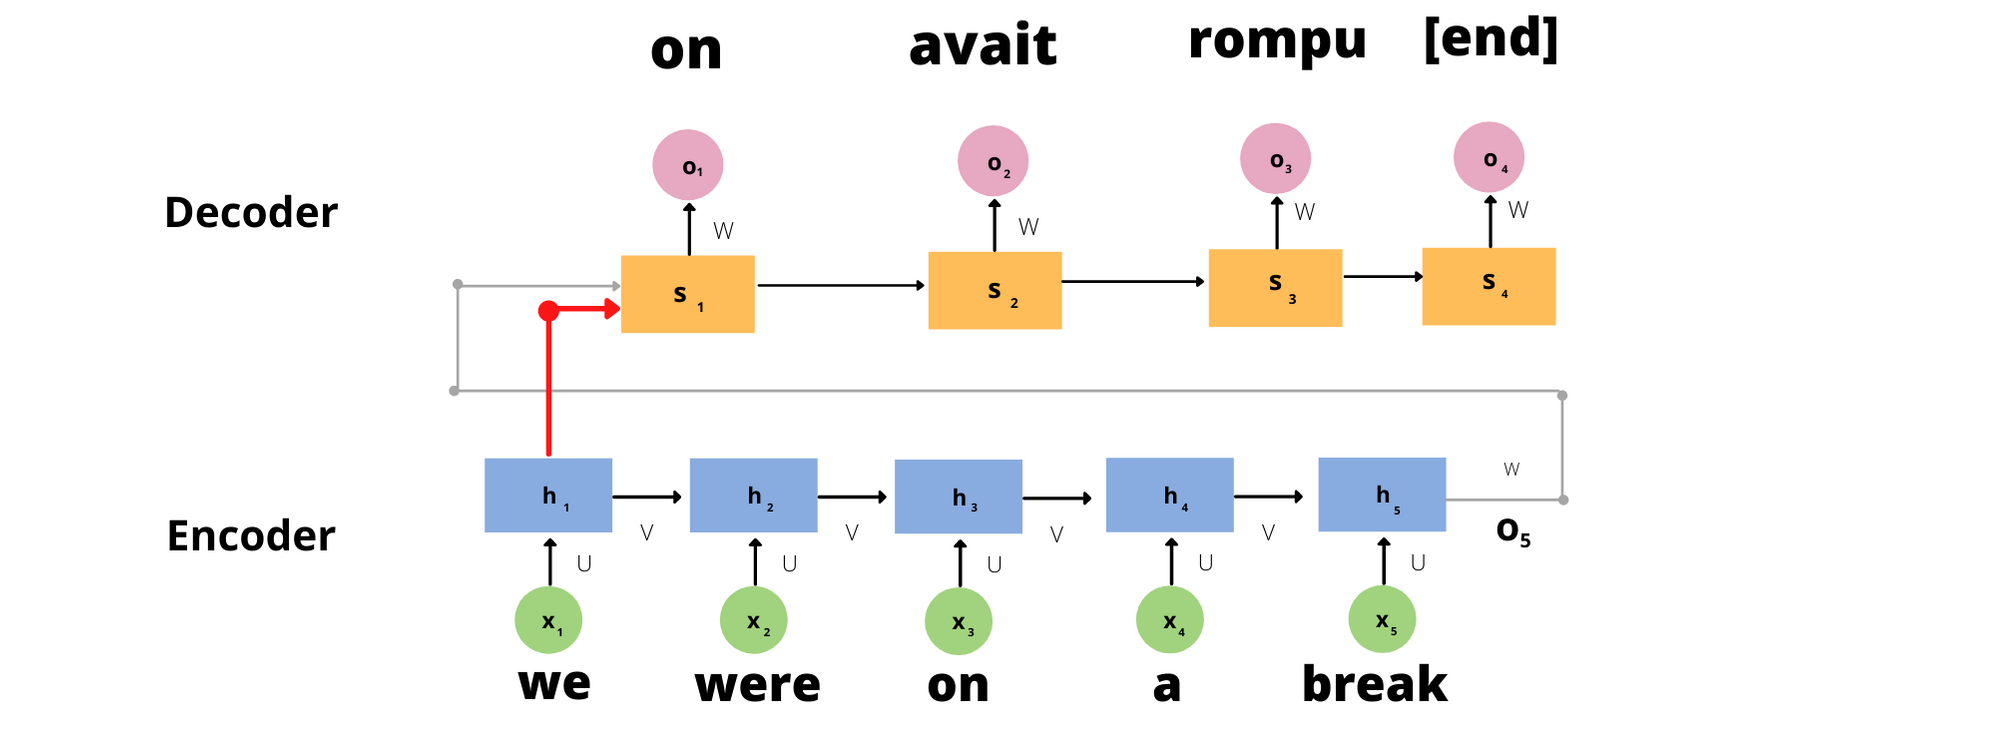
\includegraphics[width = 13cm]{img/attn_intuiton1.png}
% \end{textblock}
}
\only <2> {
% \begin{textblock}{0.15}(0.03, 0.4)
        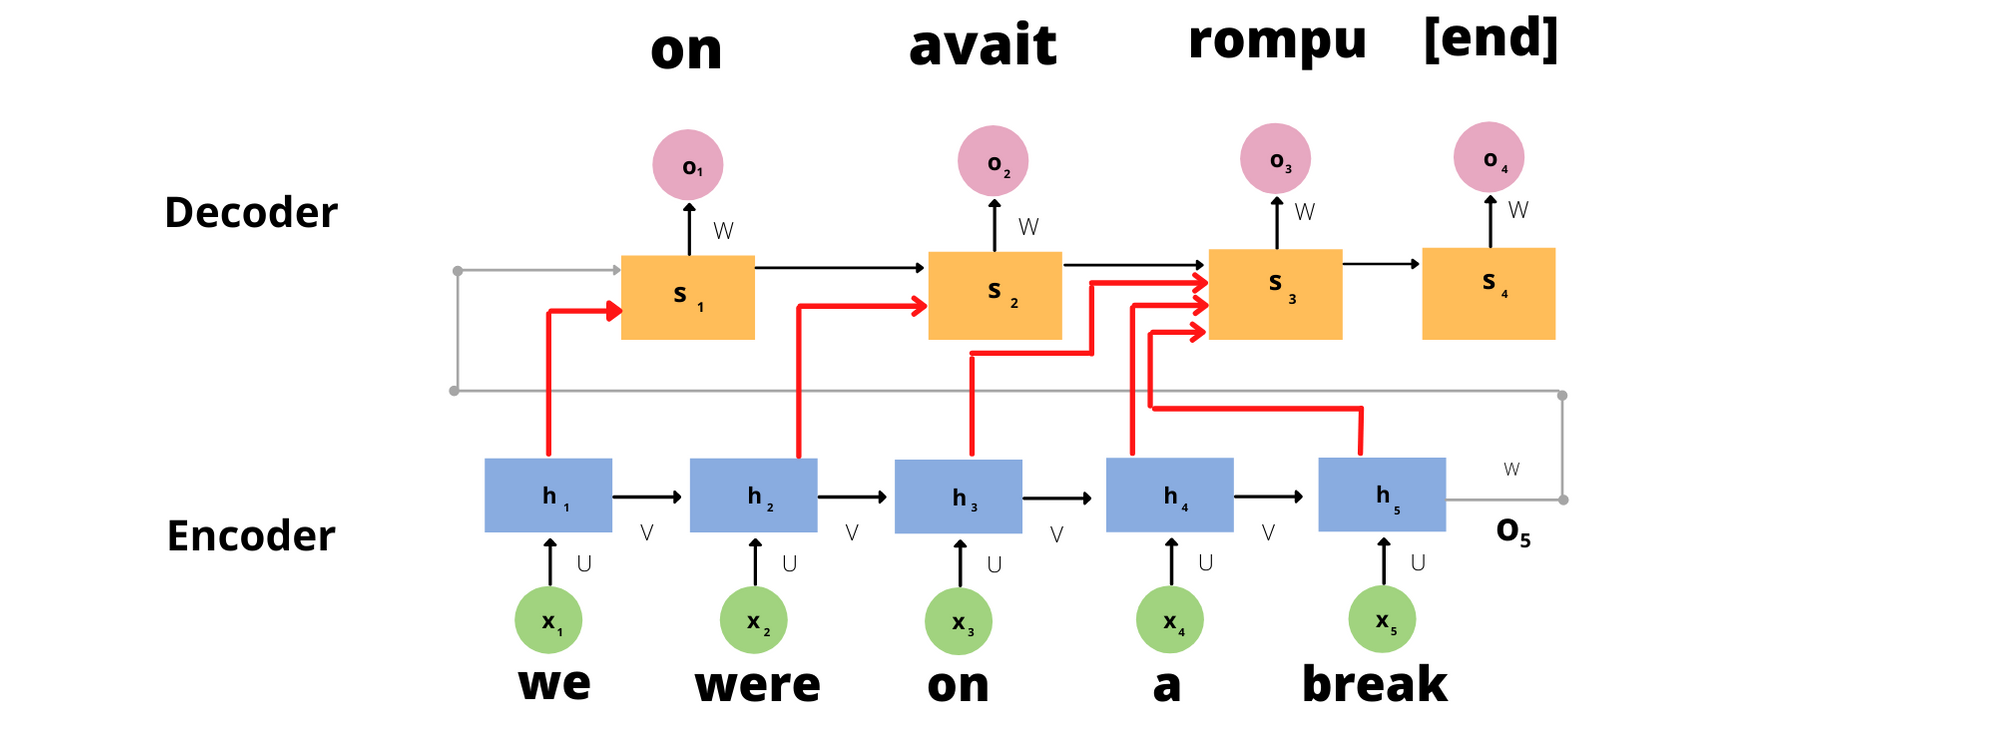
\includegraphics[width = 13cm]{img/attn_intuiton2.png}
% \end{textblock}
}
\only <3> {
% \begin{textblock}{0.15}(0.03, 0.45)
        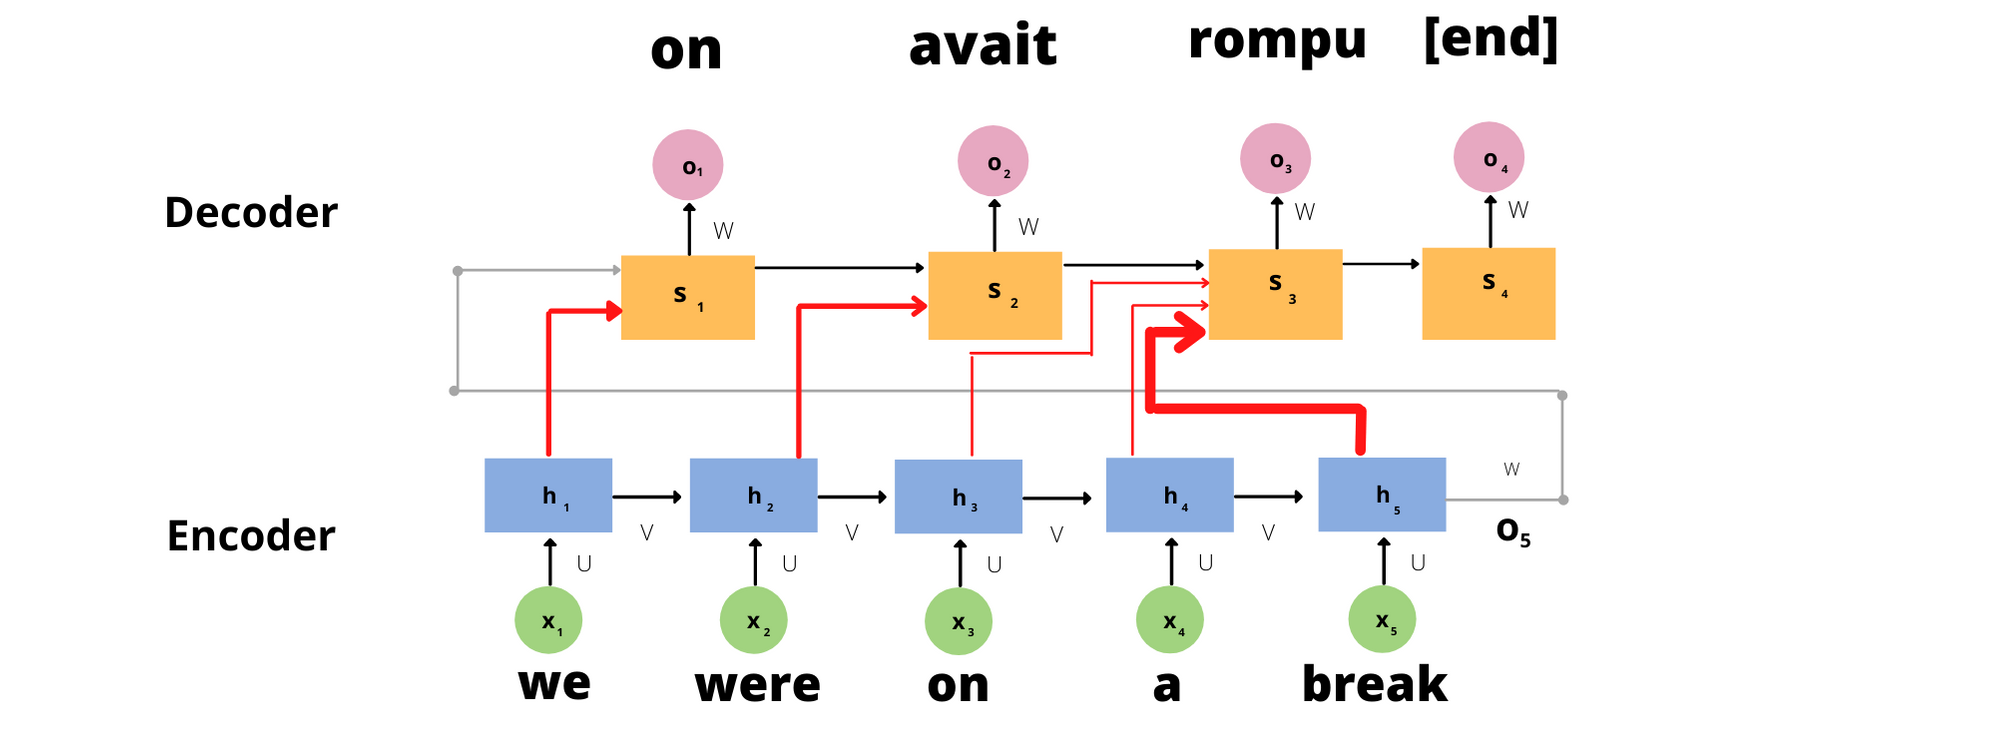
\includegraphics[width = 13cm]{img/attn_intuiton3.png}
% \end{textblock}
}
\end{frame}
\begin{frame}{Attention Modules} %%%%
\vspace{0.3cm}\\
    In other words, attention allows a direct interaction between different token positions by introducing a \tetxbf{weighted average} of the previous RNN layers into the next one.
\centering
\only <1> {
% \begin{textblock}{0.15}(0.03, 0.4)
        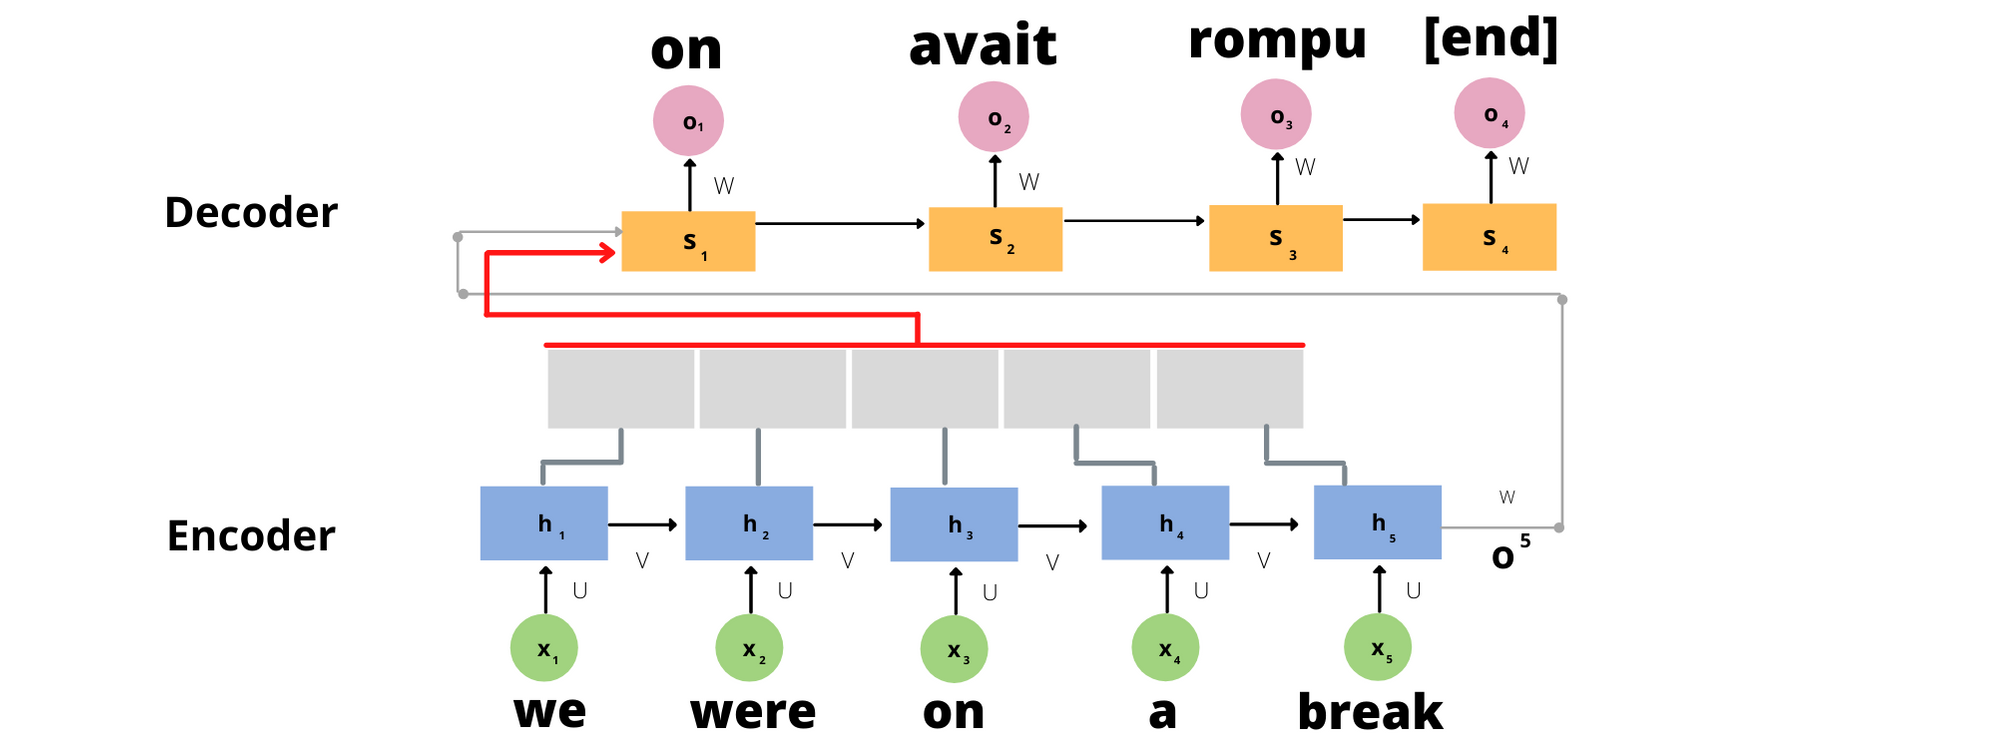
\includegraphics[width = 13cm]{img/attn_layer1.png}
% \end{textblock}
}
\only <2> {
% \begin{textblock}{0.15}(0.03, 0.4)
        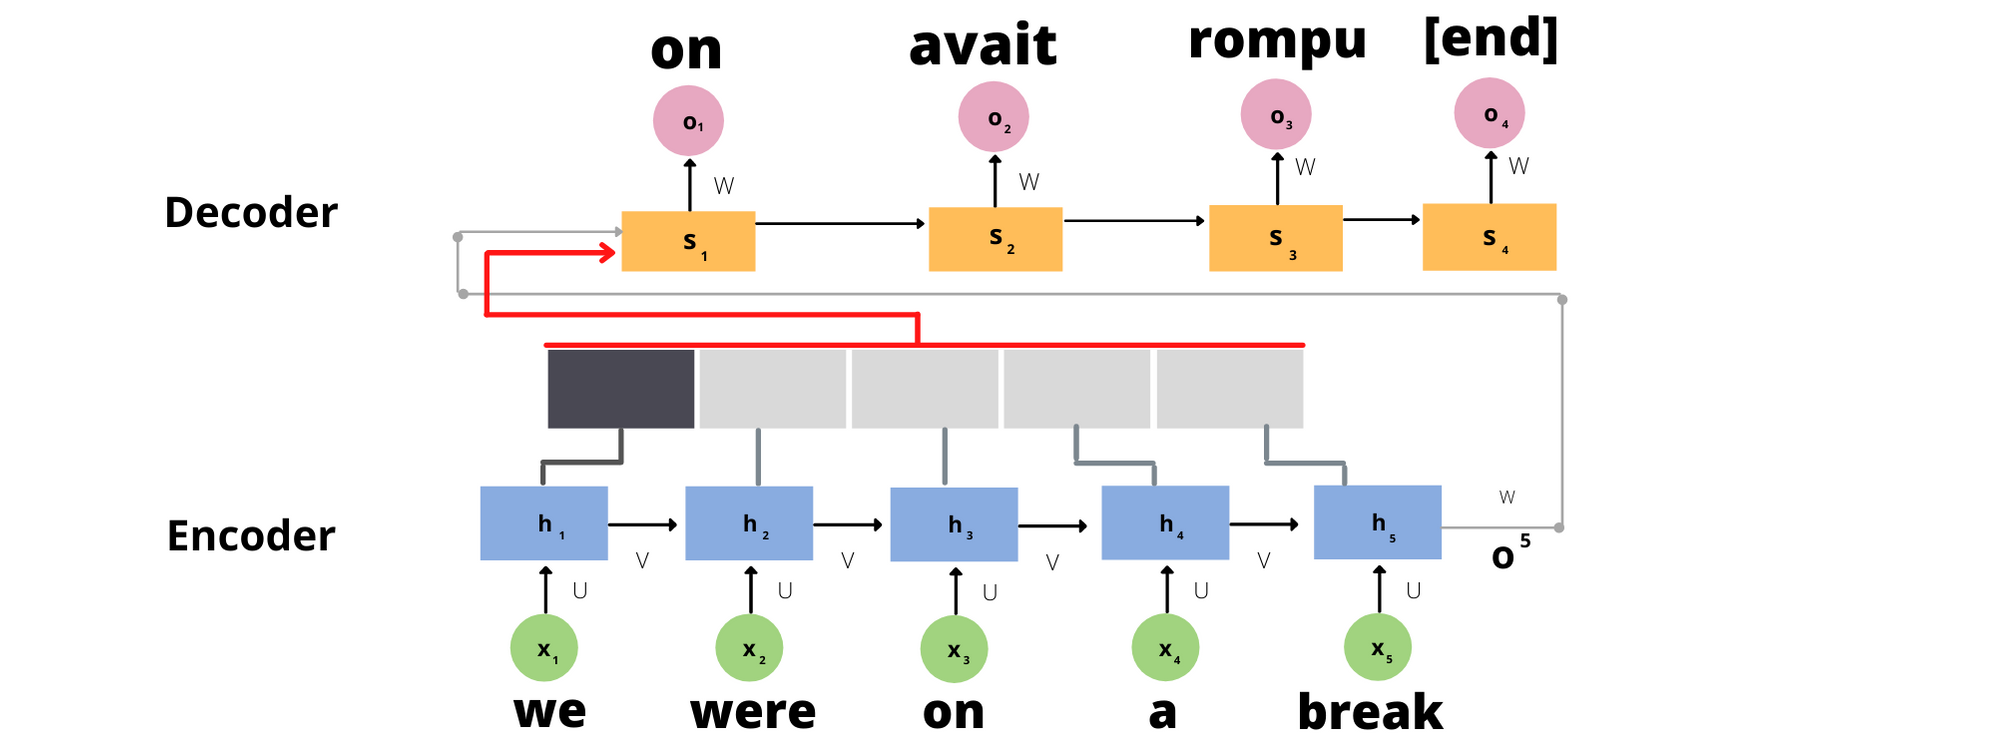
\includegraphics[width = 13cm]{img/attn_layer2.png}
% \end{textblock}
}
\only <3> {
% \begin{textblock}{0.15}(0.03, 0.4)
        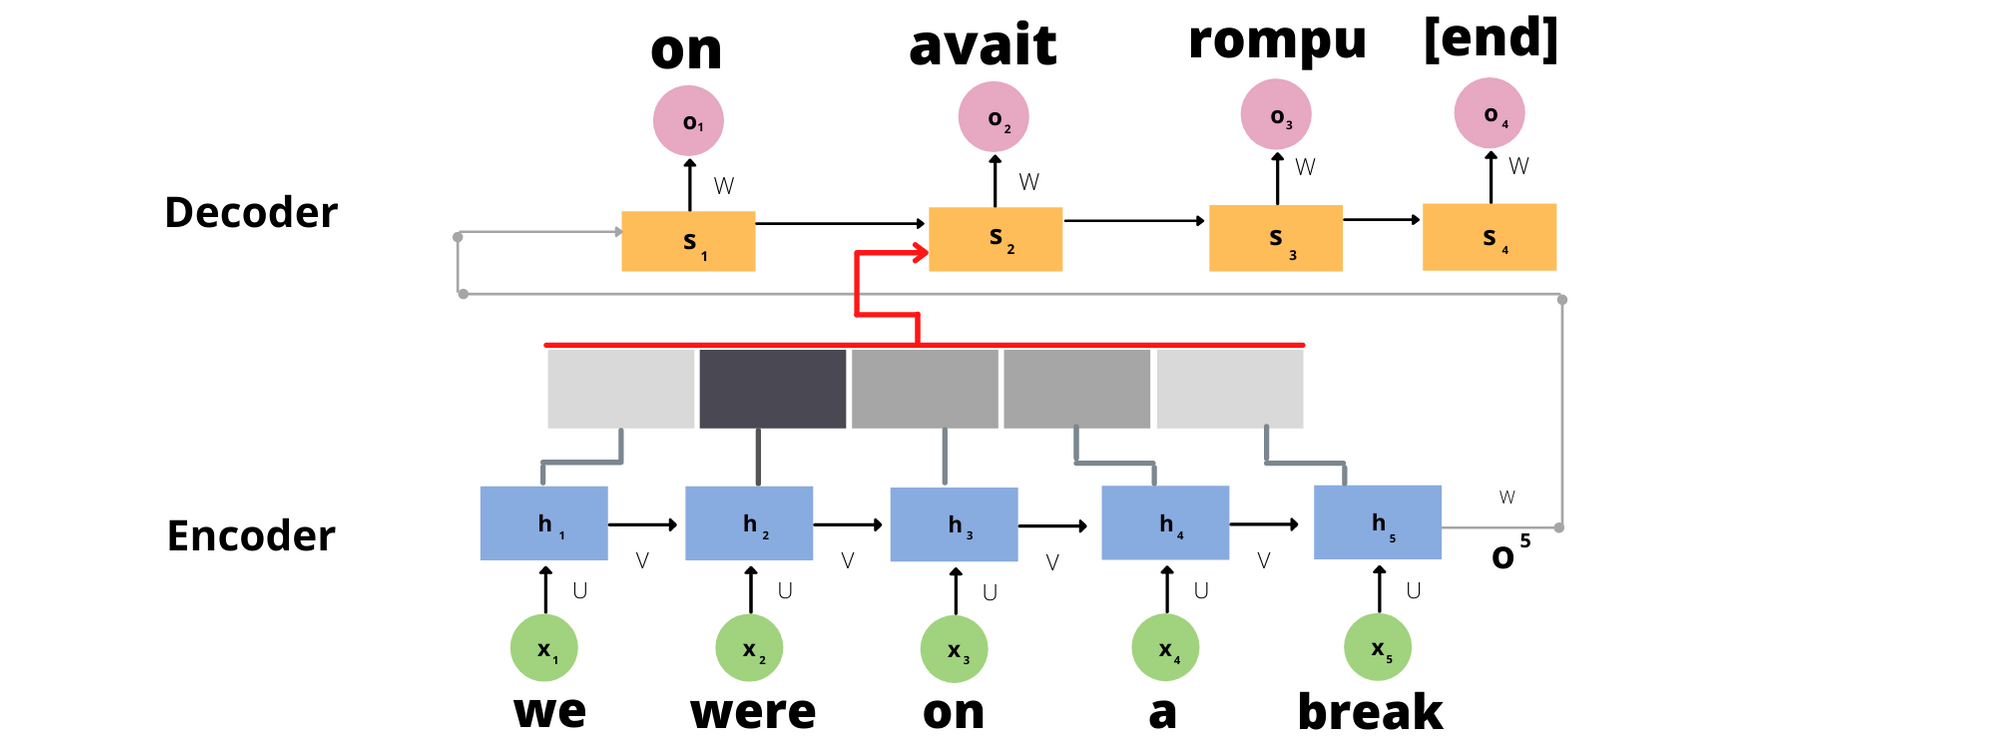
\includegraphics[width = 13cm]{img/attn_layer3.png}
% \end{textblock}
}
\only <4> {
% \begin{textblock}{0.15}(0.03, 0.4)
        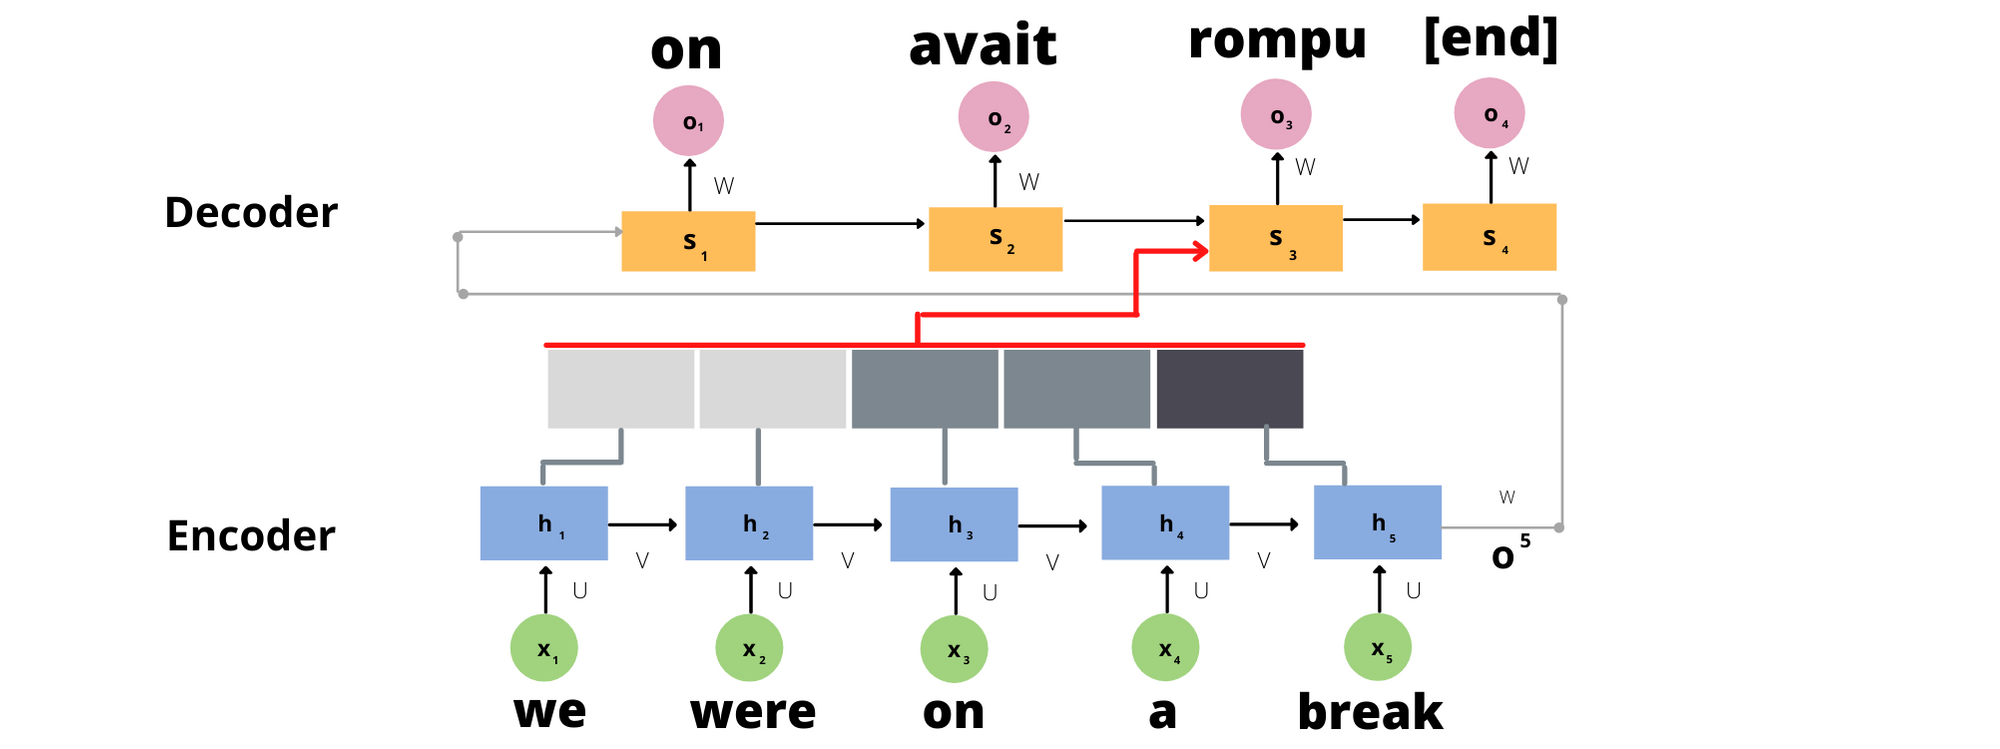
\includegraphics[width = 13cm]{img/attn_layer4.png}
% \end{textblock}
}
\end{frame}

\iffalse
\begin{frame}{Attention Modules}
\begin{columns}[onlytextwidth]
    \begin{column}{0.50\textwidth}
    We end up with a structure that resembles a \textbf{matrix}. The attention scores encode pairwise dependencies.\\
    \only <2,3,4,5,6> {More generally, we will refer to \textbf{queries (q)}, \textbf{values (v)} and \textbf{(keys (k))}. In this case we have:
    $$ A(q,K,V) = softmax(score(q,K))V$$
    $$score(s_t,h_i) = v_a^Ttanh(W_a[s_t,h_i])$$
    with learnable $v_a$ and $W_a$. Both $k,v=h_i$ come from the input RNN, while $q=s_t$ comes from the output. }
    \end{column}
\end{columns}
\only <1>{
\begin{textblock}{0.5}(0.55, 0.15)
        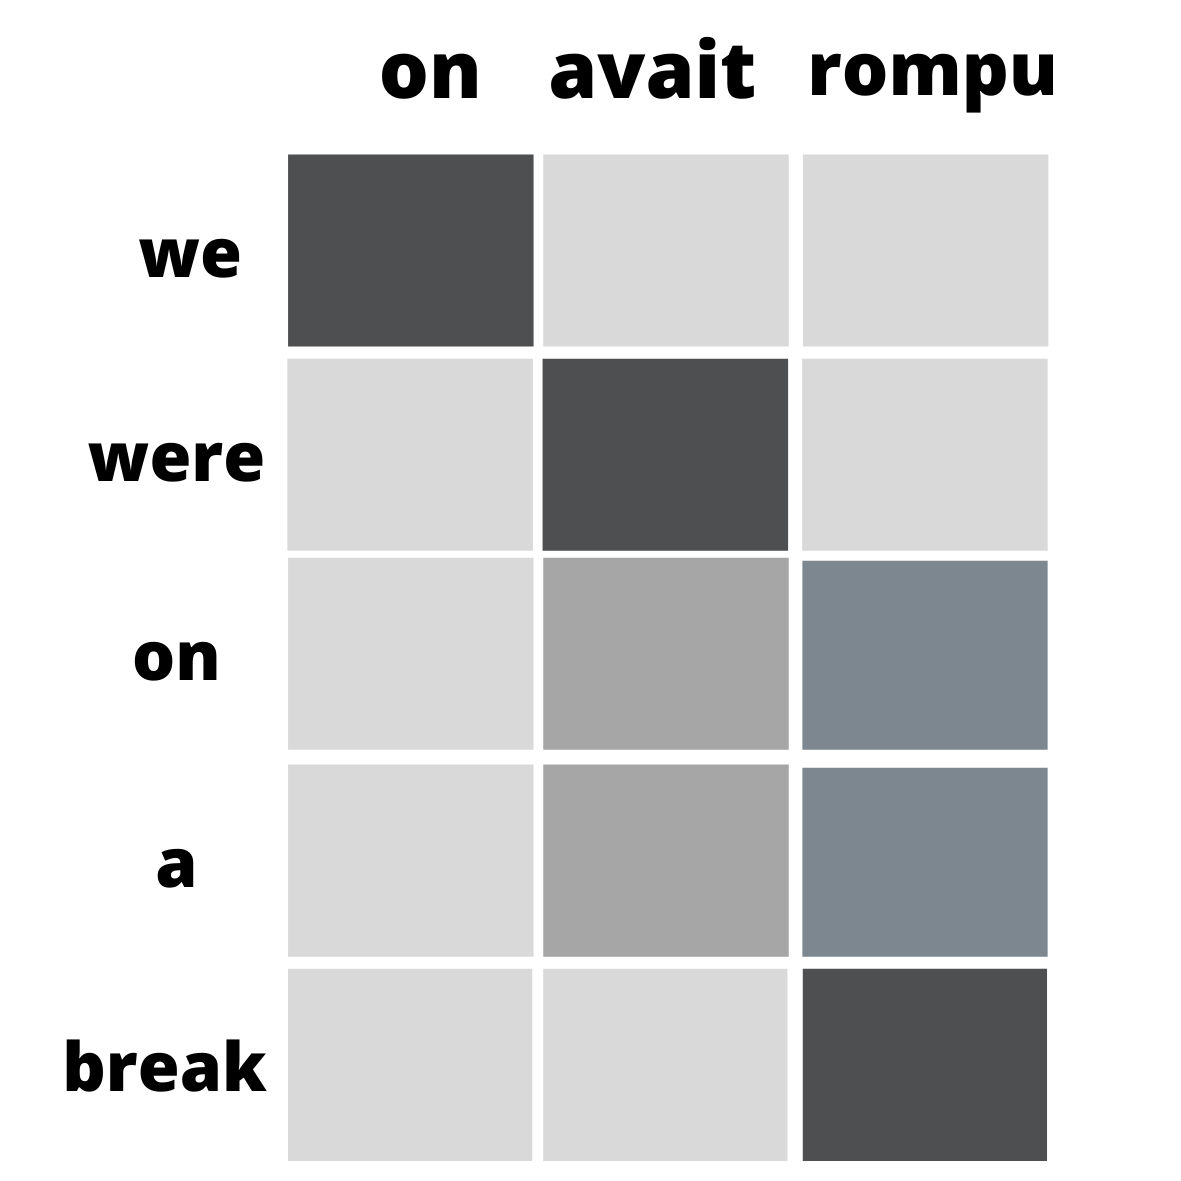
\includegraphics[width = 6cm]{img/attn_matrix.png}
\end{textblock}}
\only <2>{
\begin{textblock}{0.5}(0.55, 0.15)
        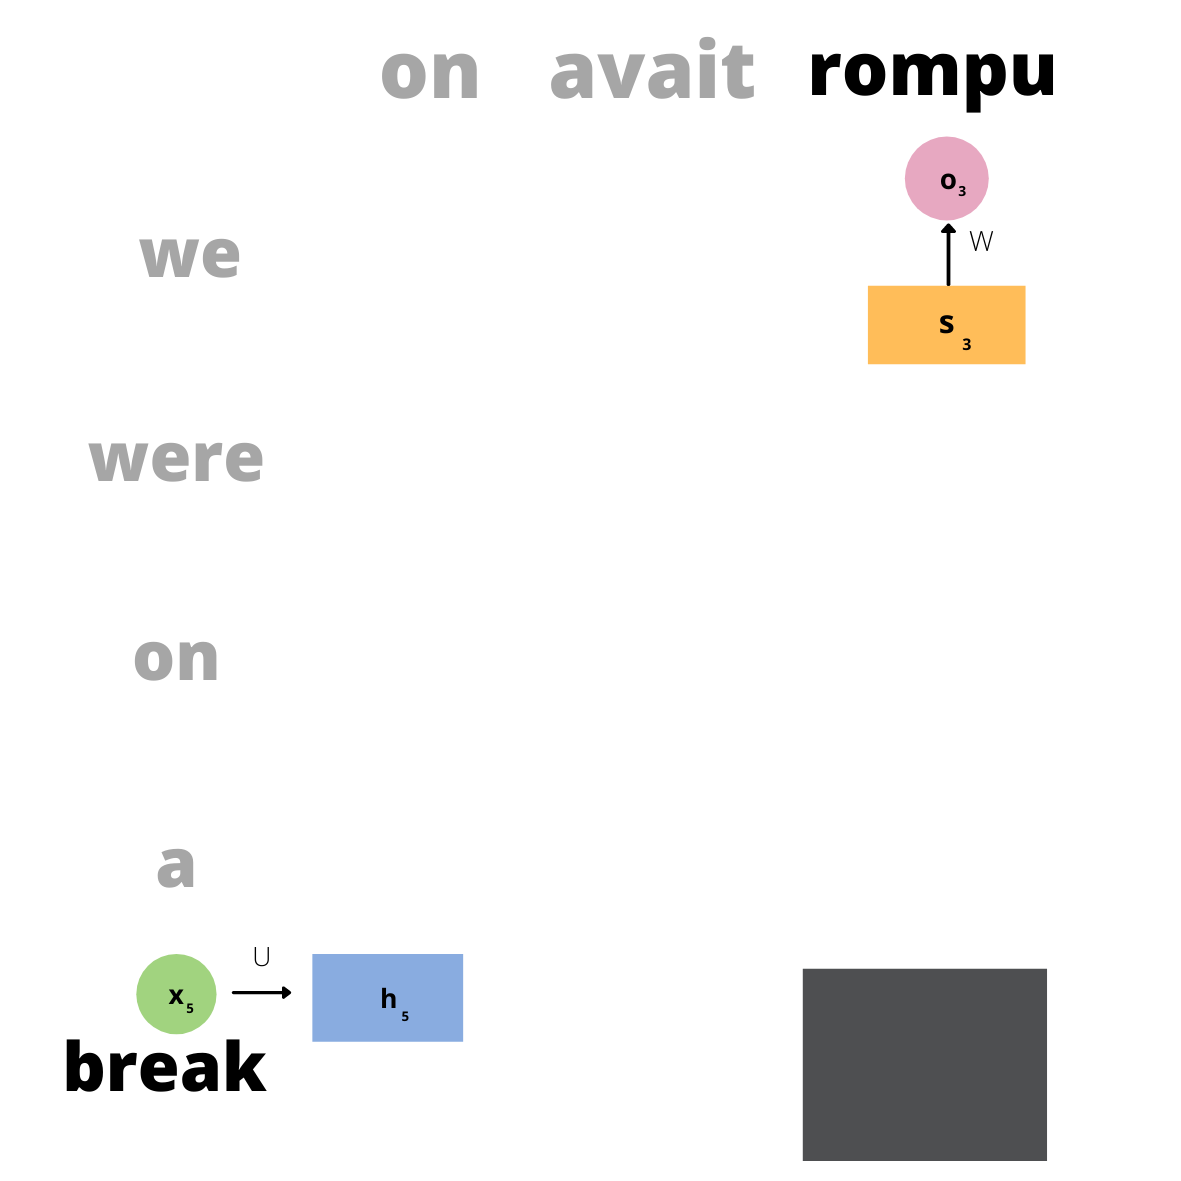
\includegraphics[width = 6cm]{img/attn_structure1.png}
\end{textblock}}
\only <3>{
\begin{textblock}{0.5}(0.55, 0.15)
        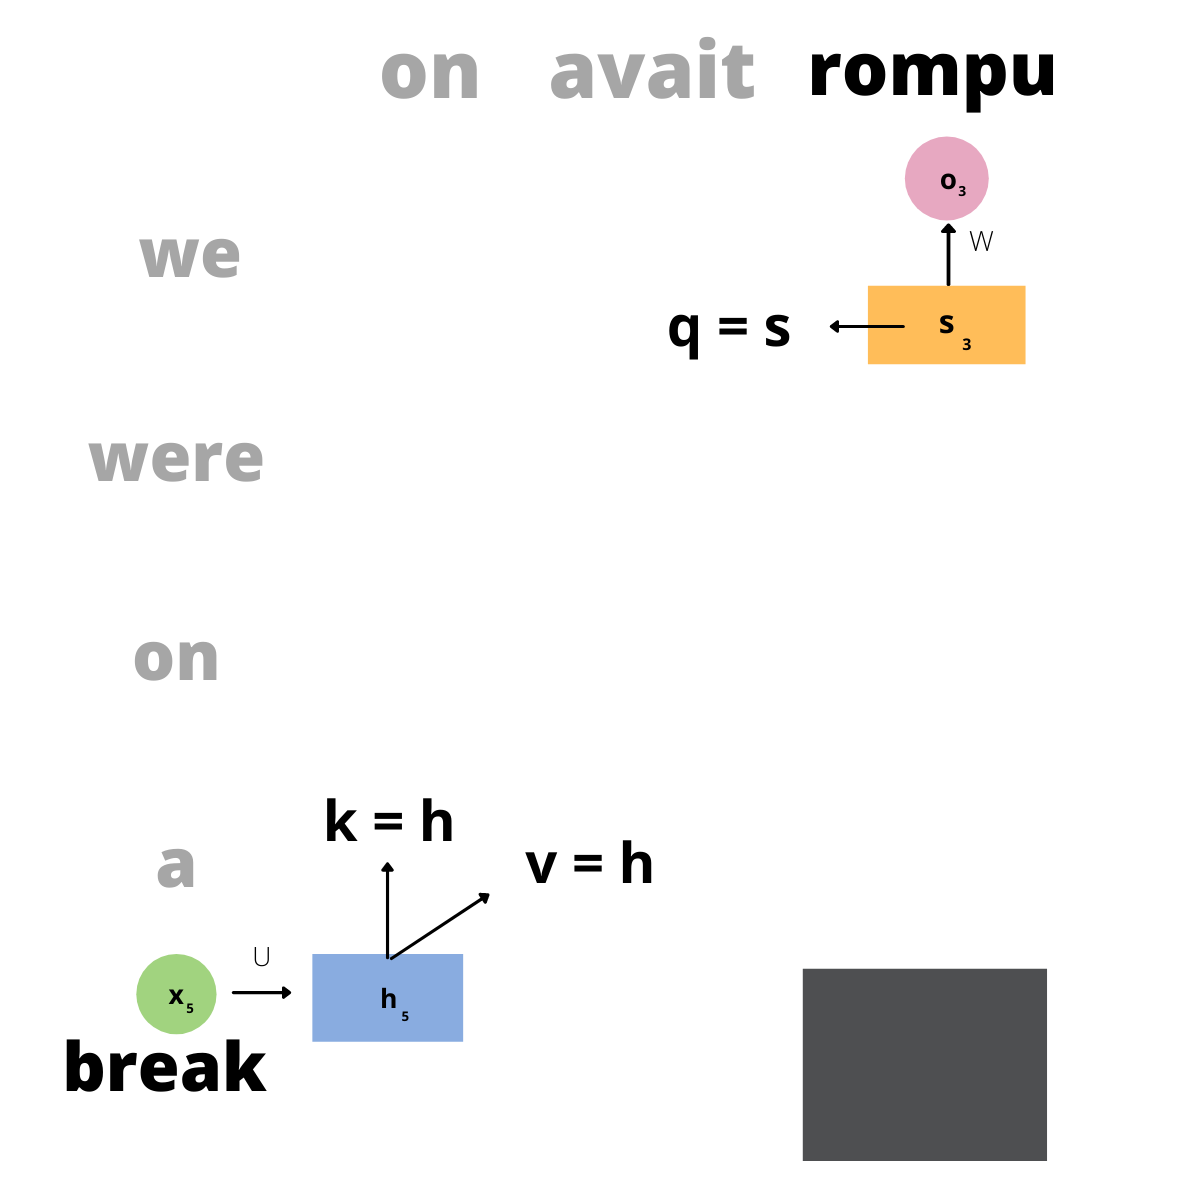
\includegraphics[width = 6cm]{img/attn_structure2.png}
\end{textblock}}
\only <4>{
\begin{textblock}{0.5}(0.55, 0.15)
        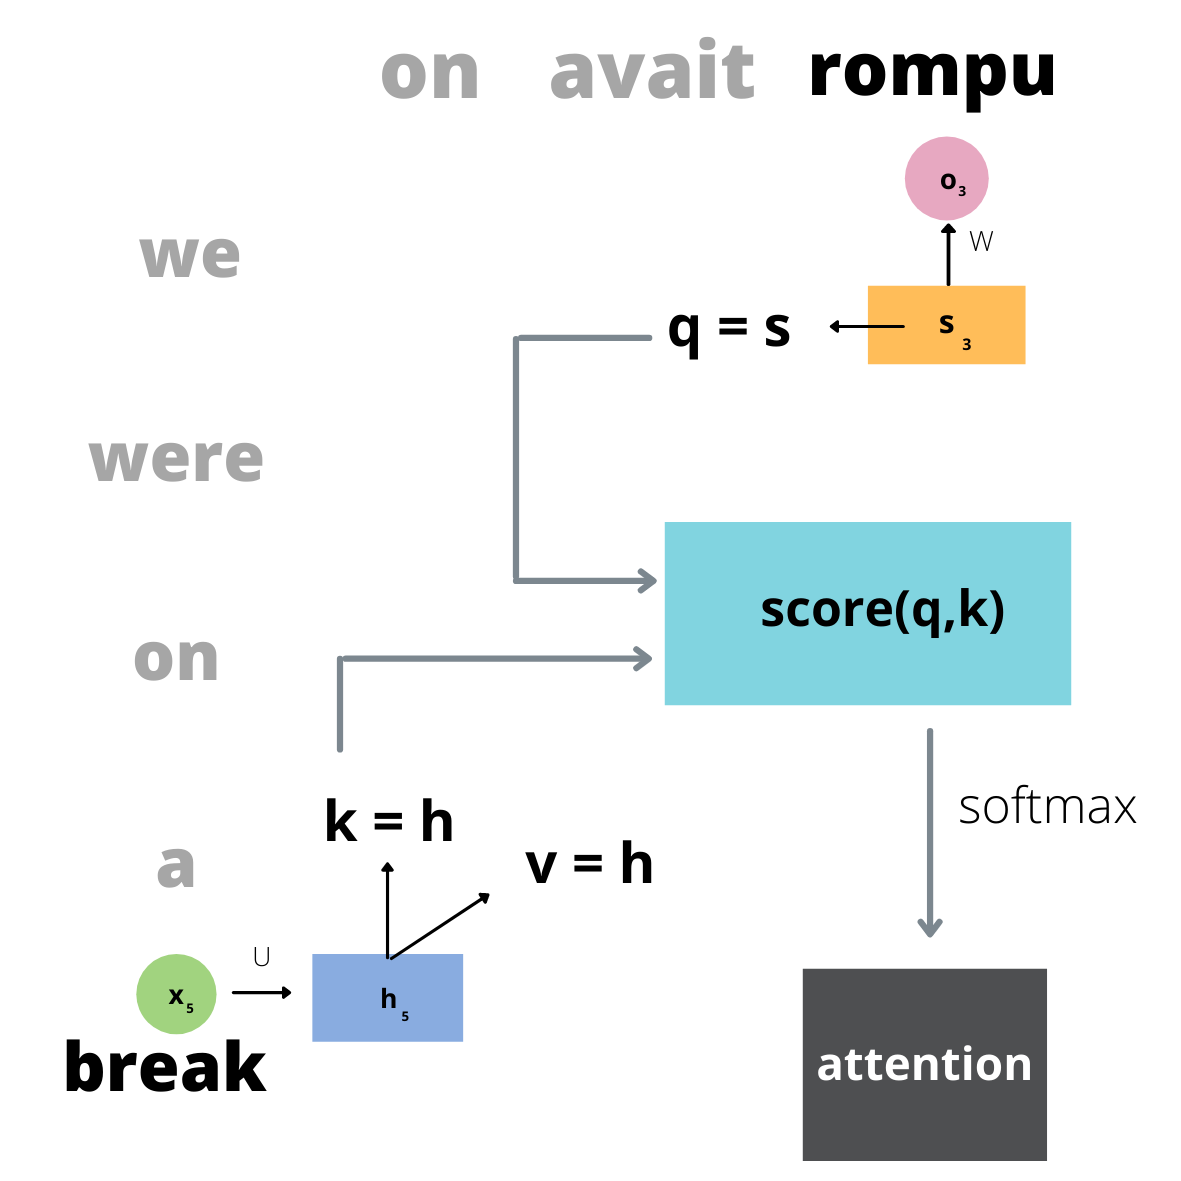
\includegraphics[width = 6cm]{img/attn_structure3.png}
\end{textblock}}
\only <5>{
\begin{textblock}{0.5}(0.55, 0.15)
        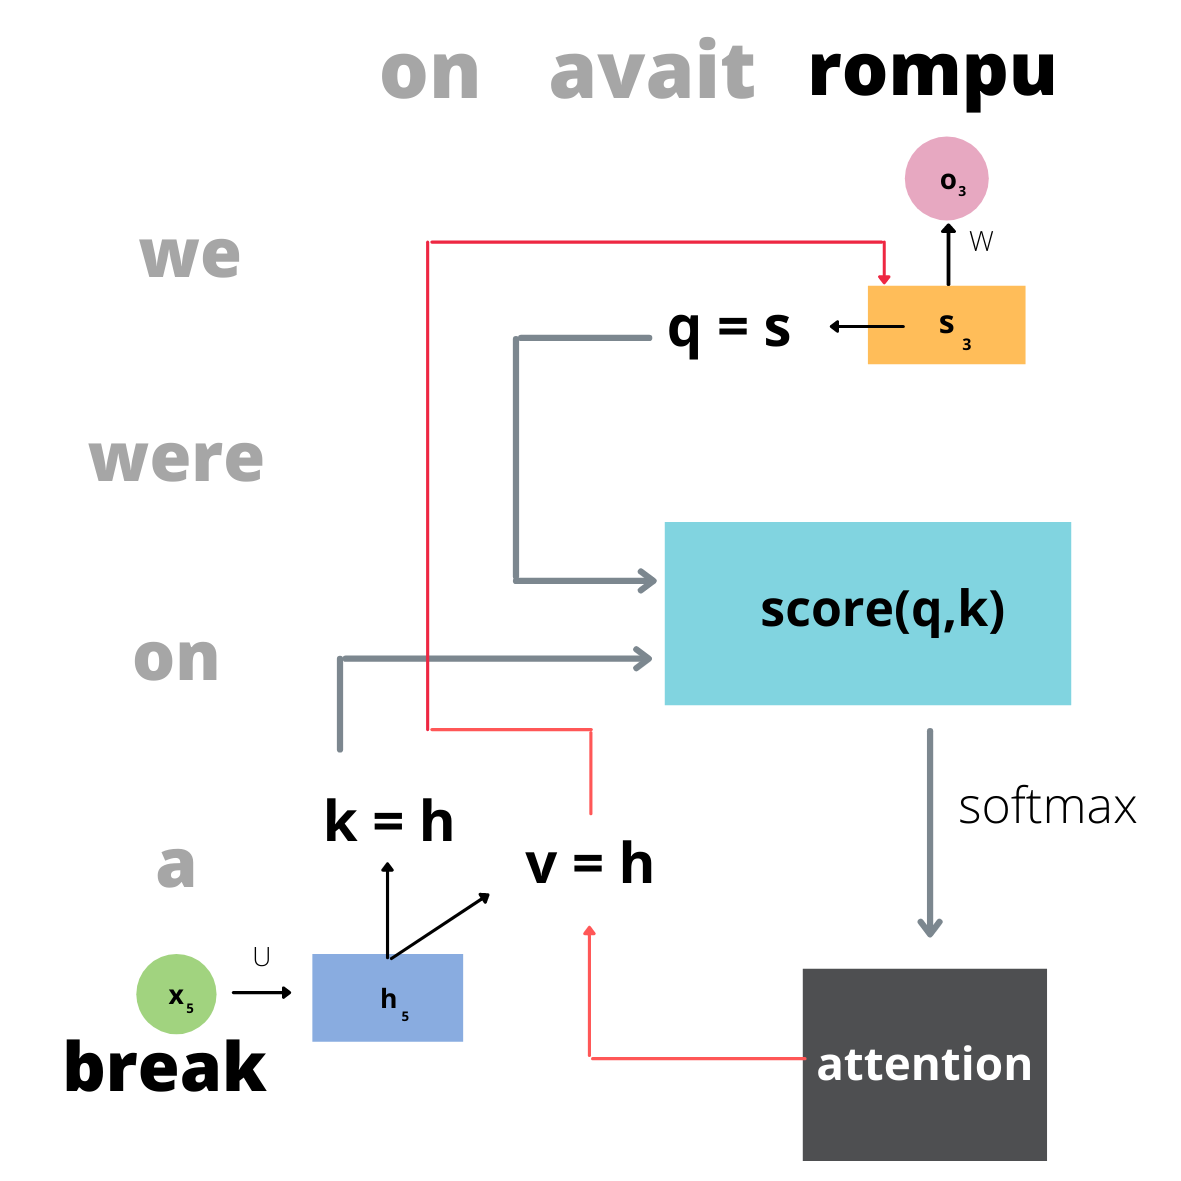
\includegraphics[width = 6cm]{img/attn_structure4.png}
\end{textblock}}
\only <6>{
\begin{textblock}{0.5}(0.5, 0.15)
        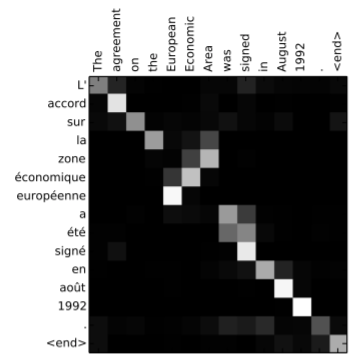
\includegraphics[width = 6cm]{img/att2.png}
\end{textblock}}
\end{frame}
\fi

\begin{frame}{Attention Modules}
\begin{columns}[onlytextwidth]
    \begin{column}{0.50\textwidth}
    We end up with a structure that resembles a \textbf{matrix}. The attention scores encode pairwise dependencies.\\
    \only <2,3,4,5,6> {More generally, we will refer to \textbf{queries (q)}, \textbf{values (v)} and \textbf{(keys (k))}. In this case we have:
    $$ A(q,K,V) = softmax(score(q,K))V$$
    $$score(s_t,h_i) = v_a^Ttanh(W_a[s_t,h_i])$$
    with learnable $v_a$ and $W_a$. Both $k,v=h_i$ come from the input RNN, while $q=s_t$ comes from the output. }
    \end{column}
    \begin{column}{0.50\textwidth}
        \centering
\only <1>{
% \begin{textblock}{0.5}(0.55, 0.15)
        \includegraphics[width = 6cm]{img/attn_matrix.png}
% \end{textblock}
}
\only <2>{
% \begin{textblock}{0.5}(0.55, 0.15)
        \includegraphics[width = 6cm]{img/attn_structure1.png}
% \end{textblock}
}
\only <3>{
% \begin{textblock}{0.5}(0.55, 0.15)
        \includegraphics[width = 6cm]{img/attn_structure2.png}
% \end{textblock}
}
\only <4>{
% \begin{textblock}{0.5}(0.55, 0.15)
        \includegraphics[width = 6cm]{img/attn_structure3.png}
% \end{textblock}
}
\only <5>{
% \begin{textblock}{0.5}(0.55, 0.15)
        \includegraphics[width = 6cm]{img/attn_structure4.png}
% \end{textblock}
}
\only <6>{
% \begin{textblock}{0.5}(0.5, 0.15)
        \includegraphics[width = 6cm]{img/att2.png}
 %\end{textblock}
}
\end{column}
\end{columns}
\end{frame}

%\section{Transformers}
\subsection{The Transformers module}
%\begin{frame}
%    \frametitle{Table of contents}
%    \tableofcontents[currentsubsection]
%\end{frame}

\begin{frame}{Attention in Transformers}
\begin{columns}[onlytextwidth]
    \begin{column}{0.50\textwidth}
    \textbf{Self-attention}: an attention network applied to the same sequence.
    \vspace{0.15cm}
    
    \textbf{Multi-head attention}, that is, $h$ attention layers running in parallel.\vspace{0.15cm}
    
    \textbf{There is no longer a recurrent network involved.}\\
\only<1,2,3,4,5>{
    
    $$score(q,K_i) = \displaystyle \frac{q^TK_i}{\sqrt{d_k}} $$
    
    \\ $Q$, $K$ and $V$ are computed from input/output using \textbf{weight matrices} $W_q, W_K$ and $W_V$
    }
    \only<6>{
    Afterwards, the contextualised token for the $j$-th token in the sequence becomes  \\
    $$ z_j = \sum^C_{i=1} score(q,K_j) v_j = S^T V $$
    }
    \end{column}
    \begin{column}{0.50\textwidth}
        \centering
\only <1>{
% \begin{textblock}{0.5}(0.51, 0.19)
    \includegraphics[width = 6cm]{img/self_attn1.png}
% \end{textblock}
}
\only <2>{
% \begin{textblock}{0.5}(0.51, 0.19)
    \includegraphics[width = 6cm]{img/multihead.png}
% \end{textblock}
}
\only <3>{
% \begin{textblock}{0.5}(0.51, 0.19)
    \includegraphics[width = 6cm]{img/self_attn2.png}
% \end{textblock}
}
\only <4>{
% \begin{textblock}{0.5}(0.51, 0.19)
    \includegraphics[width = 6cm]{img/self_attn3.png}
% \end{textblock}
}
\only <5>{
% \begin{textblock}{0.5}(0.51, 0.19)
    \includegraphics[width = 6cm]{img/self_attn4.png}
% \end{textblock}
}
\only <6>{
% \begin{textblock}{0.5}(0.51, 0.19)
    \includegraphics[width = 6cm]{img/self_attn5.png}
% \end{textblock}
}
\end{column}
\end{columns}
\end{frame}

%\subsection{Structure}
\begin{frame}{The Transformer}
\only <1>{
\begin{columns}[onlytextwidth]
    \begin{column}{0.50\textwidth}
    Transformers are a novel architecture that \textbf{gets rid of any recurrency}, thus relying solely on \textbf{attention modules}. % \cite{transformer}. 
    They have the following advantages:
    \begin{itemize}
        \item They allow for \textbf{parallelisation}.
        \item They are \textbf{flexible}, thus allowing its use on a wide variety of tasks. They only need to be pre-trained once and then they can be fine-tuned on specific tasks.
    \end{itemize}
    \end{column}
    \begin{column}{0.50\textwidth}
        \centering
        \includegraphics[width = \textwidth]{img/transformer.png}
    \end{column}
\end{columns}
}
\only <2>{
    \centering
    \includegraphics[width = 11.1cm]{img/att.png}
\footnote{\url{https://lilianweng.github.io/lil-log/2018/06/24/attention-attention.html#a-family-of-attention-mechanisms}}}
\end{frame}

\iffalse
\begin{frame}{Attention in Transformers}
\begin{columns}[onlytextwidth]
    \begin{column}{0.50\textwidth}
    Their novelty in terms of attention architecture is:\\
    The use of \textbf{scaled dot-product} score function:
    \vspace{0.15cm}
    $$score(q,K_i) = \displaystyle \frac{q^TK_i}{\sqrt{d_k}} $$ \\
    The use of \textbf{multi-head attention}, that is, $h$ attention layers running in parallel.\vspace{0.15cm}\\
    $Q$, $K$ and $V$ are computed from input/output using \textbf{weight matrices} $W_q, W_K$ and $W_V$.
    \end{column}
\end{columns}
\only <1>{
\begin{textblock}{0.5}(0.51, 0.19)
        \includegraphics[width = 6cm]{img/self_attn1.png}
\end{textblock}}
\only <2>{
\begin{textblock}{0.5}(0.51, 0.19)
        \includegraphics[width = 6cm]{img/self_attn2.png}
\end{textblock}}
\only <3>{
\begin{textblock}{0.5}(0.51, 0.19)
        \includegraphics[width = 6cm]{img/self_attn3.png}
\end{textblock}}
\only <4>{
\begin{textblock}{0.5}(0.51, 0.19)
        \includegraphics[width = 6cm]{img/self_attn4.png}
\end{textblock}}
\only <5>{
\begin{textblock}{0.5}(0.51, 0.19)
        \includegraphics[width = 6cm]{img/self_attn5.png}
\end{textblock}}
\end{frame}
\fi

\subsection{Popular Transformer-based LMs (BERT and GPT)}

\begin{frame}{Popular Transformer-based LMs}
    \begin{figure}
        \centering
        \includegraphics[width=\textwidth]{img/transformer-flavors.png}
        %\includegraphics[width = 6.5cm, height=2cm]{img/gpt0-sentiment-neuron.png}
        \caption{Source: \href{https://t.co/aYfnVKPDjT}{Transformers tutorial, by Lucas Beyer (Google Brain)}}
        \label{fig:enter-label}
    \end{figure}
\end{frame}


%\begin{frame}{GPT}
%\begin{columns}[onlytextwidth]
%    \begin{column}{0.4\textwidth}
%    \textbf{G}enerative \textbf{P}re\textbf{T}raining are a series of language models \cite{gpt} from OpenAI. 
%    \only<1>{They are said to use the decoder part of the transformer since their pre-training step consists in predicting the tokens from a sequence one by one (\textbf{Next word prediction}) (the attention heads involved in the prediction are those coming from previous tokens, hence they are unidirectional).}
%    \only<2>{\vspace{0.15cm} \\
%    The resulting LM can then be fine-tuned for specific NLP tasks, although they are mostly used for \textbf{language generation}.}
%    \end{column}
%\end{columns}
%\only<1>{
%\begin{textblock}{0.5}(0.42, 0.2)
%        \includegraphics[width = 6.9cm]{img/gpt.png}
%\end{textblock}}
%\only<2>{
%\begin{textblock}{0.5}(0.42, 0.22)
%        \includegraphics[width = 6.9cm]{img/gpt_tunning.png}
%\end{textblock}
%}
%\end{frame}


%\begin{frame}{GPT}
%     OpenAI has, since 2018, released larger and improved versions of the model. Their latest conversational model \textbf{ChatGPT} (experimental release), has gained popular attention \footnote{Visualisation from: \url{https://businessolution.org/gpt-3-statistics/}}.
%     \begin{textblock}{0.05}(0.1, 0.32)
%        \includegraphics[width = 10.5cm]{img/gpt_timeline.png}
%    \end{textblock}
%\end{frame}


%\begin{frame}{BERT}
%\begin{columns}[onlytextwidth]
%    \begin{column}{0.54\textwidth}
%    \textbf{B}idirectional \textbf{E}ncoder \textbf{R}epresentations from \textbf{T}ransformers is a large language model from Google.  % \cite{bert}\footnote{Visualising attention: \url{https://huggingface.co/exbert/}}.
%    Its pre-training relies on a joint \textbf{masked LM} (15\% of tokens) and \textbf{next sentence prediction} (i.e., discriminating between sentences that are next to one another in a corpus from ones that are not)\footnote{Visualisation from: \url{http://jalammar.github.io/illustrated-bert/}}. It is \textbf{bidirectional} since the token predictions do use information from ``future'' tokens, hence why it is considered an autoencoder model.
%    \end{column}
%\end{columns}
%\begin{textblock}{0.5}(0.55, 0.2)
%        \includegraphics[width = 5.8cm]{img/bert_MLM.png}
%\end{textblock}
%\end{frame}


%\begin{frame}{BERT}
    %BERT achieved state of the art results in several tasks, including question answering, text classification and natural language understanding (when it was released).
    %\begin{textblock}{0.05}(0.1, 0.42)
    %    \includegraphics[width = 10.5cm]{img/bert_tunning.png}
    %\end{textblock}
%\end{frame}


% \subsection{Main variations}

%\begin{frame}{Main variations}
%    There are many different variations of LMs based on transformers, let's have a look at some of them \footnote{Source of explanations: \url{https://huggingface.co/docs/transformers/model_summary}}:
    
%    \vspace{0.1cm} \\ \textbf{Sequence-to-sequence models (full transformer)}:
%    \\ These models take the whole transformer architecture. The most used are BART (Facebook, \cite{bart}) and T5 (Google, \cite{t5}), which use pre-traning processes thar are similiar to those of BERT.
%    \vspace{0.1cm} \\ \textbf{Lighter BERT variations}:
%    \vspace{0.05cm} \\- ALBERT (Google) \cite{albert}: smaller embedding size, memory sharing tricks and NSP replaced  by sentence ordering prediction.
%    \vspace{0.05cm} \\- RoBERTa (Facebook) \cite{roberta}: different masking at each epoch, larger batches, no NSP and filling max length, different tokenisation.
%    \vspace{0.05cm} \\- DistilBERT (HuggingFace) \cite{distilbert}: a smaller model trained to replicate BERT token probabilities (no NSP).
%\end{frame}


\subsection{Ethical Concerns}
\begin{frame}{Ethical Concerns with LMs}
Huge language models can be extremely dangerous % \cite{parrot}
:\\ They come at a \textbf{strong environmental cost}. \\
\\ They are usually trained on data that is \textbf{biased}, encoding \textbf{racism} and \textbf{sexism} in them.\\
It's \textbf{hard to track} and interpret them due to their size. This type of large models have oppened whole new areas of research, like BERTology % \cite{bertology}
, where the goal is to understand LMs inner behaviour.
\begin{columns}[onlytextwidth]
    \begin{column}{0.60\textwidth}
    \vspace{0.1cm}\\
    It is important to use this technology \textbf{carefully}, always assessing the possible negative outcomes. 
    \\Bigger is not always better!
    \end{column}
\end{columns}
\includegraphics[width = 3.2cm]{img/warning.png}
\end{frame}

\begin{frame}{In a Nutshell}
    \begin{itemize}
        \item \textbf{Language models} are used as a departing point for many NLP applications.
        \item They are trained with variations of \textbf{word prediction} and consuming a lot of data.
        \item \textbf{RNNs} exploit the sequential nature of data by being applied in order to each input word.
        \item \textbf{Attention} improve RNNs by allowing the model to encode complex semantics.
        \item And they are used in \textbf{Transformers} for building faster and larger models.
        \item Nevertheless, we need to be careful when we use these models since they can be \textbf{harmful} for certain demographic groups and the environment.
    \end{itemize}
\end{frame}

% ------------------------------------------------------------------------------------
% area cristobaleana

\section{Current trends in transformer-based models}
\begin{frame}
    \frametitle{Table of contents}
    \tableofcontents[currentsection]
\end{frame}


% 4.2 Arbol de modelos (decoder-only, encoder-only, end-dec). Pointer a descripción formal de las arquitecturas en pseudocódigo.
\subsection{LLM evolution}
\begin{frame}{}  % no estoy seguro de este título, fue por poner algo. Cristóbal: no título at all!
    \begin{figure}
        \centering
        %\includegraphics[width=\textwidth]{img/llm-evo-tree.png}
        \includegraphics[width=10.5cm, height=8.0cm]{img/llm-evo-tree.png}
        \caption{The sentiment neuron adjusting its value on a character-by-character basis. Source: \url{https://openai.com/research/unsupervised-sentiment-neuron}}
        \label{fig:enter-label}
    \end{figure}
\end{frame}


% GPT-0: the sentiment neuron
\subsection{GPT series}
\begin{frame}{GPT-0: The sentiment neuron (2017)}  
    % The sentiment neuron...
   Training on a significant text corpus on the task to predict the next token (LM), can we learn valuable representations for another task?

   Yes! A single ``sentiment neuron'' may control the sentiment of the generated text.
   
   Context: an era previous to the one in which Transformers took over as a de-facto architecture in sequence models.
    \begin{figure}
        \centering
        \includegraphics[width=\textwidth]{img/gpt0-sentiment-neuron.png}
        %\includegraphics[width = 6.5cm, height=2cm]{img/gpt0-sentiment-neuron.png}
        \caption{The sentiment neuron adjusting its value on a character-by-character basis. Source: \href{https://openai.com/research/unsupervised-sentiment-neuron}{Learning to generate reviews and
discovering sentiment}}
        \label{fig:enter-label}
    \end{figure}
\end{frame}

% GPT-1:
\begin{frame}{GPT-1: Decoder-only transformer (2018)}  
   OpenAI exploits and doubles the efforts on the idea that a base model can learn powerful, general representations. Transformer became a game changer on scale training! A multi-task (explicit) adaptation recipe was formed via formatting the input as a token sequence and reusing the pre-trained model.

    \begin{figure}
        \centering
        \includegraphics[width = 8.8cm, height=4.2cm]{img/gpt1-downstream-tasks.png}
        \caption{(left) Transformer decoder-only base model trained on the simple task of predicting the next token. (right) Input transformations into a token sequence to be processed by the base model, followed by a downstream layer (linear + softmax). Source: \href{https://s3-us-west-2.amazonaws.com/openai-assets/research-covers/language-unsupervised/language_understanding_paper.pdf}{Improving Language Understanding by Generative Pre-Training (GPT1 paper)}}
        \label{fig:enter-label}
    \end{figure}
\end{frame}

% GPT-2.a:
\begin{frame}{GPT-2: Prompt era unlocked (2018)}  
    \begin{figure}
        \centering
        %\includegraphics[width=\textwidth]{img/prompt-era-ex2.png}
        \includegraphics[width = 9.2cm, height=6.6cm]{img/prompt-era-ex2.png}
        \caption{Make your model look like a document to auto-complete translation without explicit supervision, with no downstream task layer at all. Source: \href{https://d4mucfpksywv.cloudfront.net/better-language-models/language_models_are_unsupervised_multitask_learners.pdf}{Language Models are Unsupervised Multitask Learners (GPT2 paper)}.}
        \label{fig:enter-label}
    \end{figure}
\end{frame}

% GPT-2.b:
\begin{frame}{GPT-2: Fake it till you make it (2018)}  
   GPT-2 kicked off the era of prompting over fine-tuning. No explicit supervision. Make your model look like a document, so the inherent task is performed by taking the model and asking to complete the document (prompt era unlocked). There is no further training or gradient updates \footnote{Some articles explore the idea of an explicit gradient-like update of the parameters when doing prompting.} to its parameters. 

    \begin{figure}
        \centering
        %\includegraphics[width=\textwidth]{img/prompt-era-ex1.png}
        \includegraphics[width = 5.5cm, height=2.2cm]{img/prompt-era-ex1.png}
        \caption{\href{https://arxiv.org/pdf/2206.07682.pdf}{Emergent Abilities of Large Language Models} (Source)}
        \label{fig:enter-label}
    \end{figure}
\end{frame}

% GPT-2.c:
\begin{frame}{GPT-2: Scalability payoffs (2018)}  
   Scalability proves useful for powerful and general representations when performing zero-shot transfer.
   In a nutshell, \textbf{How do we exploit general capabilities without intervening with the model head—the re-purpose layer for downstream tasks—in the context of predicting the next token?} Scaling + prompting

    \begin{figure}
        \centering
        \includegraphics[width=\textwidth]{img/gpt2-zero-shot-performance.png}
        \caption{Zero-shot performance of a base model trained on WebText as a function of model size (117M-345M-762M-1542M parameters) in 4 different NLP tasks. Each task is evaluated on a benchmark dataset and compared with SOTA-specific models at that time, 2018-2019. Source: \href{https://cdn.openai.com/better-language-models/language_models_are_unsupervised_multitask_learners.pdf}{Language Models are Unsupervised Multitask Learners (GPT2 paper)}.}
        \label{fig:enter-label}
    \end{figure}
\end{frame}



%\subsection{GPT assistant training pipeline}
% ChatGPT.a: more than a LM. Explain quickly each stage of the model.
\begin{frame}{ChatGPT: more than a LM (2022)}
    \begin{figure}
        \centering
        \includegraphics[width=\textwidth]{img/gpt-assistant-pipeline.png}
        \caption{Slide from the talk "The State of GPT", by Andrej Karpathy (2023).}
        \label{fig:enter-label}
    \end{figure}
\end{frame}

% ChatGPT.b: supervised fine-tuning
\begin{frame}{ChatGPT: Supervised Finetuning}
    \begin{column}{0.50\textwidth}
        \begin{figure}
            \centering
            \includegraphics[width = 3.2cm, height=5.1cm]{img/sft-chatgpt.png}
            \caption{source: \href{phttps://arxiv.org/pdf/2106.09685.pdf}{Training language models to follow instructions with human feedback}}
            \label{fig:enter-label}
        \end{figure}
    \end{column}
    \begin{column}{0.50\textwidth}
        \begin{figure}
            \centering
            \includegraphics[width = 6.0cm, height=8.2cm]{img/sft-chatgpt-instructions.png}
            \label{fig:enter-label}
        \end{figure}
    \end{column}
\end{frame}


% chatgpt.c: more than a lm. explain quickly each stage of the model.
\begin{frame}{ChatGPT: Reward Modeling}
    \begin{column}{0.40\textwidth}
        \begin{figure}
            \centering
            \includegraphics[width = 3.2cm, height=5.4cm]{img/sft-chatgpt-rm.png}
            \caption{\href{phttps://arxiv.org/pdf/2106.09685.pdf}{Training language models to follow instructions with human feedback}}
            \label{fig:enter-label}
        \end{figure}
    \end{column}
    \begin{column}{0.50\textwidth}
        \begin{figure}
            \centering
            \includegraphics[width=\textwidth]{img/sft-chatgpt-upvotes-ranking.png}
            \label{fig:enter-label}
            \caption{An example of a reward modelling dataset. Source: slide from the talk ``the state of gpt'', by Andrej Karpathy (2023).}
        \end{figure}
    \end{column}
\end{frame}

  
% chatgpt.d: more than a lm. explain quickly each stage of the model.
\begin{frame}{ChatGPT: RL from Human Feedback}
    \begin{column}{0.40\textwidth}
        \begin{figure}
            \centering
            \includegraphics[width = 3.2cm, height=5.4cm]{img/rlhf-chatgpt-diagram.png}
            \caption{\href{phttps://arxiv.org/pdf/2106.09685.pdf}{Training language models to follow instructions with human feedback}}
            \label{fig:enter-label}
        \end{figure}
    \end{column}
    \begin{column}{0.60\textwidth}
        \begin{figure}
            \caption{Reinforcement Learning from Human Feedback (Loop). Source: \href{https://huggingface.co/blog/rlhf}{Illustrating Reinforcement Learning from Human Feedback (RLHF)}}
            \centering
            \includegraphics[width=\textwidth]{img/rlhf-chatgpt.png}
            \label{fig:enter-label}
        \end{figure}
    \end{column}
\end{frame}


% 4.4 Open Source: LoRA, Quantization, lograr correct modelos en notebooks.
% Sobre..
\subsection{The Open Source Community}
\begin{frame}{Open Source models are faster}  % no estoy seguro de este título, fue por poner algo
    Meta LLaMA-13B Leak to the public, March 03/2023 → Fine-tuning with ChatGPT conversation (prompt-response) → Alpaca-13B (2 weeks apart, budget \$USD500) → Fine-tuning with 70k user-shared ChatGPT (ShareGPT.com) conversations → Vicuna-13B (1 week apart, budget \$USD150).
    \begin{figure}
        \centering
        \includegraphics[width = 9.5cm, height=4.2cm]{img/vicuna-gpt-performance.png}
        %\includegraphics[width=\textwidth]{img/vicuna-gpt-performance.png}
        %\caption{TODO...}
        \label{fig:enter-label}
    \end{figure}
\end{frame}


\begin{frame}{Constraints + Community = Innovations.}
    \begin{column}{0.50\textwidth}
        \begin{itemsize}
            \item Finetuning an LLM is prohibitive for the majority of individuals.
            \vspace{0.1cm}
            \item Finetuning a model requires saving an entire copy.
            \vspace{0.1cm}
            \item Finetuning could downgrade model performance on other tasks.
            \vspace{0.1cm}
            \item LoRA uses low-rank matrices to update and freeze the original parameters. Modular. Easy to share.
        \end{itemsize}
    \end{column}
    \begin{column}{0.50\textwidth}
        \begin{figure}
            \centering
            \includegraphics[width = 5.4cm, height=4.2cm]{img/lora-finetuning.png}
            \caption{Freeze the pre-trained model weights and inject trainable rank decomposition matrices (A and B) into each layer of the Transformer architecture. Source: \href{phttps://arxiv.org/pdf/2106.09685.pdf}{LoRA: Low-Rank Adaptation of Large Language Models}}
            \label{fig:enter-label}
        \end{figure}
    \end{column}
\end{frame}

%\begin{frame}{Constraints + Community = innovations 2.}
%\only <1>{
%\begin{columns}[onlytextwidth]
%    \begin{column}{0.50\textwidth}
%    Transformers are a novel architecture that \textbf{gets rid of any recurrency}, thus relying solely on \textbf{attention modules} \cite{transformer}. They have the following advantages:
%    \begin{itemize}
%        \item They allow for \textbf{parallelisation}.
%        \item They are \textbf{flexible}, thus allowing its use on a wide variety of tasks. They only need to be pre-trained once and then they can be fine-tuned on specific tasks.
%    \end{itemize}
%    \end{column}
%\end{columns}
%\begin{textblock}{0.5}(0.51, 0.05)
    %%\includegraphics[width = \textwidth]{img/transformer.png}
    %\begin{figure}
    %    \centering
    %    \includegraphics[width = 5.7cm, height=4.2cm]{img/lora-finetuning.png}
    %    \caption{Freeze the pre-trained model weights and inject trainable rank decomposition matrices (A and B) into each layer of the Transformer architecture. Source: \href{phttps://arxiv.org/pdf/2106.09685.pdf}{LoRA: Low-Rank Adaptation of Large Language Models}}
        %\label{fig:enter-label}
    %\end{figure}
%   \end{textblock}}
%\only <2>{\begin{textblock}{0.05}(0.05, 0.19)
%    \includegraphics[width = 11.1cm]{img/att.png}
%\end{textblock}
%\end{frame}

% \subsection{Modelos autoregresivos en imágenes: PixelRNN - PixelCNN}
\subsection{Autoregresive models on images: PixelRNN and PixelCNN}

\begin{frame}{PixelRNN (Van den Oord et al. 2016)}
  \begin{column}{0.50\textwidth}
        \begin{itemsize}
            \item Typically, we saw NLP examples linked to autoregressive models, but it is also possible to generate images.
            \vspace{0.1cm}
            \item PixelRNN is a generative model used for image generation, mainly focused on generating images one pixel at a time.
            \vspace{0.1cm}
            \item Compute a hidden state for each pixel that depends on hidden states and RGB values from the left and above (LSTM recurrence). 
            $$
            h_{x,y}=f(h_{x-1, y}, h_{x,y-1}, W)
            $$
            \vspace{0.1cm}
            \item Problem: Very slow during training and testing; $N\times N$ image requires $2N-1$ sequential steps.
        \end{itemsize}
    \end{column}
    \begin{column}{0.50\textwidth}
        \begin{figure}
            \centering
            \includegraphics[width = 4.5cm, height=4.5cm]{diapositivas/img/pixelrnn.png}
            \caption{The blue pixel only depends on the light blue pixels (left and above). Predict red, blue, and green (0-255) using the hidden states for the previous and current pixels. Source: \href{https://arxiv.org/abs/1601.06759}{Pixel Recurrent Neural Networks}}
            \label{fig:enter-label}
        \end{figure}
    \end{column}
\end{frame}



\begin{frame}{PixelCNN (Van den Oord et al. 2016)}
  \begin{column}{0.50\textwidth}
        \begin{itemsize}
            \item PixelCNN extends the idea of capturing pixel dependencies by using masked convolutions, which restrict the network's access to information about future pixels, ensuring a causal generation process.
            \vspace{0.1cm}
            \item Training is faster than PixelRNN; we can parallelise convolutions since context region values are known in advance.
            \vspace{0.1cm}
            \item Generation is still slow; we must proceed sequentially, generating pixel by pixel.
            \vspace{0.1cm}
        \end{itemsize}
    \end{column}
    \begin{column}{0.50\textwidth}
        \begin{figure}
            \centering
            \includegraphics[width = 4.5cm, height=4.5cm]{diapositivas/img/pixelcnn.png}
            \caption{The black square depicts a predicted pixel that uses convolution to capture previous pixel dependencies but ensures that it does not see subsequent pixels. The task is to predict the following pixel so the masked, or causal convolution, trims that portion of the local context. Source: \href{https://arxiv.org/abs/1601.06759}{Pixel Recurrent Neural Networks}}
            \label{fig:enter-label}
        \end{figure}
    \end{column}
\end{frame}


%Quitar de comentarios apenas se agregue alguna referencia 
% \bibliography{../capitulos/referencias} %Bibliografía
% \bibliographystyle{apacite}


\section{References}

\begin{frame}[allowframebreaks]
    \frametitle{References}
    % \scriptsize
    \begin{thebibliography}% {}
    \tiny{
    
        % \setbeamertemplate{bibliography item}[text]
        % \bibitem{bayes}
        % Metsis, V., Androutsopoulos, I., & Paliouras, G. (2006, July). Spam filtering with naive bayes-which naive bayes?. In CEAS (Vol. 17, pp. 28-69).
        
        % \bibitem{word2vec}
        % Mikolov, T., Chen, K., Corrado, G., & Dean, J. (2013). Efficient Estimation of Word Representations in Vector Space. ArXiv:1301.3781 [Cs]. \url{http://arxiv.org/abs/1301.3781}
        
        % \bibitem{lda}
        % Blei, D. M., Ng, A. Y., & Jordan, M. I. (2003). Latent dirichlet allocation. the Journal of machine Learning research, 3, 993-1022.
        
        %\bibitem{lsa}
        %Deerwester, S. C., Dumais, S. T., Furnas, G. W., Harshman, R. A., CA, Landauer, T. K., Lochbaum, K. E., & Streeter, L. A. (1989). United States Patent: 4839853 - Computer information retrieval using latent semantic structure (Patent No. 4839853). %\url{http://patft.uspto.gov/netacgi/nph-Parser?Sect1=PTO1&Sect2=HITOFF&d=PALL&p=1&u=%2Fnetahtml%2FPTO%2Fsrchnum.htm&r=1&f=G&l=50&s1=4839853.PN.&OS=PN/4839853&RS=PN/4839853}
        
        %\bibitem{glove}
        %Pennington, J., Socher, R., & Manning, C. (2014). Glove: Global Vectors for Word Representation. Proceedings of the 2014 Conference on Empirical Methods in Natural Language Processing (EMNLP), 1532–1543. \url{https://doi.org/10.3115/v1/D14-1162}
        
        %\bibitem{retro}
        %Faruqui, M., Dodge, J., Jauhar, S. K., Dyer, C., Hovy, E., & Smith, N. A. (2015). Retrofitting Word Vectors to Semantic Lexicons. Proceedings of the 2015 Conference of the North American Chapter of the Association for Computational Linguistics: Human Language Technologies, 1606–1615. \url{https://doi.org/10.3115/v1/N15-1184}
        
        %\bibitem{numberbatch}
        %Speer, R., Chin, J., & Havasi, C. (2017). ConceptNet 5.5: An open multilingual graph of general knowledge. Proceedings of the Thirty-First AAAI Conference on Artificial Intelligence, 4444–4451.

        \bibitem{bengio}
        Bengio, Y., Ducharme, R., Vincent, P., & Jauvin, C. (2003). A Neural Probabilistic Language Model. The Journal of Machine Learning Research, 19.

        % \bibitem{mikolov}
        % Mikolov, T., Yih, W., & Zweig, G. (2013). Linguistic Regularities in Continuous Space Word Representations. Proceedings of the 2013 Conference of the North American Chapter of the Association for Computational Linguistics: Human Language Technologies, 746–751. \url{https://www.aclweb.org/anthology/N13-1090}

        %\bibitem{calis}
        %Caliskan, A., Bryson, J. J., & Narayanan, A. (2017). Semantics derived automatically from language corpora contain human-like biases. Science, 356(6334), 183–186. \url{https://doi.org/10.1126/science.aal4230}
        
        %\bibitem{boluk}
        %Bolukbasi, T., Chang, K.-W., Zou, J. Y., Saligrama, V., & Kalai, A. T. (2016). Man is to Computer Programmer as Woman is to Homemaker? Debiasing Word Embeddings. In D. D. Lee, M. Sugiyama, U. V. Luxburg, I. Guyon, & R. Garnett (Eds.), Advances in Neural Information Processing Systems 29 (pp. 4349–4357). Curran Associates, Inc. \url{http://papers.nips.cc/paper/6228-man-is-to-computer-programmer-as-woman-is-to-homemaker-debiasing-word-embeddings.pdf}
        
        \bibitem{rnn}
        Elman, J. L. (1990). Finding structure in time. Cognitive science, 14(2), 179-211.
        
        % \bibitem{lstm}
        % Hochreiter, S., & Schmidhuber, J. (1997). Long Short-term Memory. Neural Computation, 9, 1735–1780. \url{https://doi.org/10.1162/neco.1997.9.8.1735}
        
        \bibitem{attention}
        Bahdanau, D., Cho, K., & Bengio, Y. (2016). Neural Machine Translation by Jointly Learning to Align and Translate. ArXiv:1409.0473 [Cs, Stat]. \url{http://arxiv.org/abs/1409.0473}
        
        \bibitem{transformer}
        Vaswani, A., Shazeer, N., Parmar, N., Uszkoreit, J., Jones, L., Gomez, A. N., Kaiser, Ł., & Polosukhin, I. (2017). Attention is All you Need. Advances in Neural Information Processing Systems, 30, 5998–6008. \url{https://arxiv.org/abs/1706.03762}
        
        \bibitem{bert}
        Devlin, J., Chang, M.-W., Lee, K., & Toutanova, K. (2019). BERT: Pre-training of Deep Bidirectional Transformers for Language Understanding. Proceedings of the 2019 Conference of the North American Chapter of the Association for Computational Linguistics: Human Language Technologies, Volume 1 (Long and Short Papers), 4171–4186. \url{https://doi.org/10.18653/v1/N19-1423}
        
        \bibitem{parrot}
        Bender, E. M., Gebru, T., McMillan-Major, A., & Shmitchell, S. (2021). On the Dangers of Stochastic Parrots: Can Language Models Be Too Big? Proceedings of the 2021 ACM Conference on Fairness, Accountability, and Transparency, 610–623. \url{http://faculty.washington.edu/ebender/papers/Stochastic_Parrots.pdf}

        % Parte 2: GPT series + ChatGPT (TODO CRISTÓBAL)
        \bibitem{sentiment-neuron}
        Radford, A., Jozefowicz, R., & Sutskever, I. (2017). Learning to generate reviews and discovering sentiment. arXiv 2017. arXiv preprint arXiv:1704.01444. \url{https://openai.com/research/unsupervised-sentiment-neuron}

        \bibitem{gpt1}
        Radford, A., Narasimhan, K., Salimans, T., & Sutskever, I. (2018). Improving language understanding by generative pre-training. \url{https://openai.com/research/language-unsupervised}

        \bibitem{gpt2}
        Radford, A., Wu, J., Child, R., Luan, D., Amodei, D., & Sutskever, I. (2019). Language models are unsupervised multitask learners. OpenAI blog, 1(8), 9. \url{https://cdn.openai.com/better-language-models/language_models_are_unsupervised_multitask_learners.pdf}

        % jelou
        \bibitem{meta-gradient}
        Von Oswald, J., Niklasson, E., Randazzo, E., Sacramento, J., Mordvintsev, A., Zhmoginov, A., & Vladymyrov, M. (2023, July). Transformers learn in-context by gradient descent. In International Conference on Machine Learning (pp. 35151-35174). PMLR. \url{https://proceedings.mlr.press/v202/von-oswald23a.html}

        \bibitem{gpt-instruction}
        Ouyang, L., Wu, J., Jiang, X., Almeida, D., Wainwright, C., Mishkin, P., ... & Lowe, R. (2022). Training language models to follow instructions with human feedback. Advances in Neural Information Processing Systems, 35, 27730-27744. \url{https://openai.com/research/instruction-following#sample5}

        \bibitem{lora}
        Hu, E. J., Shen, Y., Wallis, P., Allen-Zhu, Z., Li, Y., Wang, S., ... & Chen, W. (2021). Lora: Low-rank adaptation of large language models. arXiv preprint arXiv:2106.09685. \url{https://arxiv.org/abs/2106.09685}

        \bibitem{emergent-abilities}
        Wei, J., Tay, Y., Bommasani, R., Raffel, C., Zoph, B., Borgeaud, S., ... & Fedus, W. (2022). Emergent abilities of large language models. arXiv preprint arXiv:2206.07682. \url{https://arxiv.org/pdf/2206.07682.pdf}A

        \bibitem{pixelrnn}
        Van Den Oord, A., Kalchbrenner, N., & Kavukcuoglu, K. (2016, June). Pixel recurrent neural networks. In International conference on machine learning (pp. 1747-1756). PMLR.\url{https://arxiv.org/pdf/1601.06759.pdf}

    }
    \end{thebibliography}

\end{frame}



\begin{frame}
  \titlepage
\end{frame}


\end{document} 
